\documentclass[11pt,a4paper]{article}
\usepackage{fontspec}
\setmainfont{TeX Gyre Pagella}
\usepackage[a4paper,margin=2.4cm]{geometry}
\usepackage{amsmath}
\usepackage{graphicx,booktabs,float,caption,array,xcolor,longtable,threeparttable}
\usepackage{xurl}
\usepackage[hidelinks]{hyperref}
\usepackage{titlesec}
\usepackage[round,authoryear]{natbib}
\usepackage{setspace}
\setstretch{1.08}
\renewcommand{\topfraction}{0.9}
\renewcommand{\bottomfraction}{0.8}
\renewcommand{\textfraction}{0.1}
\renewcommand{\floatpagefraction}{0.75}
\setlength{\parindent}{0pt}
\setlength{\parskip}{0.55em}
\titleformat{\section}{\bfseries\Large}{\thesection}{0.8em}{}
\titleformat{\subsection}{\bfseries\large}{\thesubsection}{0.8em}{}
\captionsetup{font=small,labelfont=bf}
\urlstyle{same}
\hypersetup{pdftitle={Does a Local MP Get a Local Bonus?},pdfauthor={Tristan Hotham}}

\begin{document}
\begin{center}
{\LARGE\bfseries Does a Local MP Get a Local Bonus?\par}
\vspace{0.4em}
{\large Birthplace and the electoral performance of UK Members of Parliament, 1832 to 2024\par}
\vspace{1.2em}
{\large Tristan Hotham\par}
\vspace{0.3em}
{\small Independent researcher\\
ORCID: 0000-0003-4931-9349\\
DOI: https://doi.org/10.5281/zenodo.24092361\par}
\vspace{0.8em}
2026
\end{center}

\begin{quote}
\small
\begin{center}\textbf{Abstract}\end{center}
Voters say they prefer candidates with local roots, and since 2010 British parties have selected far more locally born candidates. Whether local roots win real votes over the long run is less clear. I link every Member of Parliament returned at the 49 UK general elections from 1832 to 2024 (31{,}737 returns) to birthplaces and constituency results, and test pre-specified hypotheses with six designs. Comparing MPs elected for the same seat, each net of their own party's national performance, an MP born within 25 km of the seat won 1.29 percentage points more of the vote (95\% CI 0.73 to 1.85; $N=14{,}580$). Three within-seat designs agree in sign: local incumbents gained 0.31 points more at re-election, a hand-over to a local successor raised the party's relative share by 0.67 points, and a local MP's retirement cost the party 0.9 points more than a non-local MP's. The bonus is the same among first-time winners and when only MPs of the same party in the same seat are compared; a lead placebo and permutation tests are null and a fake-seat placebo is close to zero. Yet local incumbents were not less likely to be defeated (+1.0 percentage points, 95\% CI -0.3 to +2.3) and did not serve longer: most margins dwarf the bonus. The estimated bonus since 2010, as localness rose, is small and uncertain. Birthplace is a proxy for roots and the design is observational: the results describe a modest, persistent electoral premium for local birth, not a decisive one.

\textbf{Keywords:} friends and neighbours voting; candidate localness; personal vote; incumbency; Members of Parliament; British elections; electoral history
\end{quote}

\section{Introduction}
``Local'' is among the most valued traits a British parliamentary candidate can have. Asked to choose between hypothetical candidates, voters prefer the one who lives in or comes from the area \citep{campbellcowley2014,campbell2019}; candidates advertise their roots on leaflets; and parties have responded. In my earlier descriptive study of all MPs since 1832, the share of MPs born within 25 km of the constituency they represent was close to a quarter at almost every general election from 1832 to 2005, and then rose to 43\% at the 2024 election \citep{hotham2026mpl}. Behind that rise lies a simple belief, held by selectors and candidates: local roots win votes.

Whether they do, in real elections and across a long span of time, is surprisingly hard to establish. Survey experiments show that voters like local candidates in principle, but they measure stated preferences over hypothetical profiles. Studies of real elections in Britain mostly use the distance between voters' and candidates' homes at a single election \citep{arzheimerevans2012,arzheimerevans2014,evans2017}, which identifies a ``friends and neighbours'' effect within a constituency but says little about whether a locally rooted MP outperforms a non-local one in aggregate, or whether that advantage is large enough to change who wins. The historical literature on the personal vote in Britain, meanwhile, focuses on incumbency and constituency service rather than on roots \citep{cain1987,gaines1998,eggersspirling2017}.

This paper asks four questions of the full population of MPs returned at UK general elections from 1832 to 2024. Do MPs born near their constituency win a higher vote share than other MPs elected for the same seat, once their party's national performance is taken into account? Do they do better at re-election, relative to their party's national swing? Are they less often defeated, and do they serve longer? And has the advantage changed as localness has become common? I answer them with six designs, written down with their robustness, placebo and heterogeneity checks before any outcome model was run.

The question matters beyond academic curiosity. If local roots win votes, parties have an electoral reason to prefer local candidates, and the rise of the local MP is partly a story about strategy. If they do not, the rise needs another explanation: changes in who comes forward, in how local parties run selections, or in the kind of people who now enter politics. The answer also bears on representation. A local MP may be valued for symbolic reasons, as one of us, or for instrumental ones, as someone who knows the area and will work for it \citep{childscowley2011,campbell2019}. Electoral rewards for localness, if they exist, are one channel through which such preferences shape who sits in Parliament.

The contribution is threefold. First, scale and span: 31{,}737 MP returns over 192 years, with birthplaces placed for 57\% of them, linked to constituency results. Second, identification: rather than comparing local and non-local candidates across seats, the main design compares MPs within the same seat, net of each party's national performance (a variant compares only MPs of the same party in the same seat), and three further designs exploit changes of MP within a seat (re-election, succession and retirement), with a lead placebo. Third, a substantive answer that distinguishes vote share from outcomes: there is a local bonus of about one percentage point, stable across robustness checks and present in each British nation (less certainly among Conservatives), but it does not reduce the chance of defeat or lengthen careers, and it is not larger in the recent era of local MPs.

\section{Background and literature}
\subsection{Friends and neighbours}
The idea that candidates draw extra support near home goes back to \citet{key1949}, who mapped the ``friends and neighbors'' vote in Southern primaries, where candidates ran strongest in and around their home counties. In American elections the effect has been traced in presidential home states \citep{lewisbeckrice1983}, as a function of distance with a steep decay \citep{gimpel2008}, as a source of identification for coattail effects \citep{meredith2013}, and in a field experiment on turnout \citep{panagopoulos2017}. Outside the United States, local ties help candidates under open-list and preferential systems in Estonia \citep{tavits2010}, Ireland \citep{goreckimarsh2012} and across proportional systems more broadly \citep{shugart2005}, and voters in at-large list systems reward their own localities \citep{fivahalse2016}.

In Britain, \citet{johnston1974} found local effects in a local election, and the electoral geography of Britain has long emphasised neighbourhood and campaign effects \citep{johnstonpattie2006}. The modern British evidence on candidate localness comes from three strands. Observational studies relate voters' party choice to the distance between their homes and candidates' homes, finding that voters are more likely to support a nearby candidate, net of party, at the 2010 general election \citep{arzheimerevans2012}, at English county council elections \citep{arzheimerevans2014} and in 2015, when the authors also coded candidates' local roots \citep{evans2017}. Survey experiments show that voters prefer candidates described as local \citep{campbellcowley2014} and that the appeal of local roots reflects expectations of behaviour, such as constituency focus, as well as group attachment \citep{campbell2019}; regional identity conditions who uses localness as a cue \citep{collignonsajuria2018}, and the effect is found in comparative experiments too \citep{harfst2024}. Normative work asks whether local presence is a form of descriptive representation worth having \citep{childscowley2011}, and voters' preferences over how MPs divide their effort between Westminster and constituency are documented by \citet{vivyanwagner2016}.

\subsection{Why would local roots win votes?}
The literature offers several mechanisms, which differ in what they predict for the British case. The first is information. Where voters know little about candidates, a local origin is a cheap cue that the candidate shares their interests, will be accessible and will defend the area \citep{shugart2005}. On this account the value of localness should be greatest where other information is scarce, and should shrink when party labels carry most of the information, as they do in British general elections. The second is social identity and affect: voters favour someone from their own place for the same reasons they favour members of other in-groups, a mechanism that \citet{campbell2019} distinguish from expectations about behaviour and find to be part, but not all, of the appeal of local roots. The third is networks and mobilisation. Candidates who grew up in an area know more people there, can call on friends and family to campaign, and may mobilise turnout among acquaintances \citep{key1949,goreckimarsh2012,panagopoulos2017}; such effects decay steeply with distance \citep{gimpel2008} and are concentrated among voters close to the candidate's home \citep{arzheimerevans2012}. The fourth is behaviour in office: local MPs may do more constituency work, which builds a personal vote over time \citep{cain1987,vivyanwagner2016}.

These mechanisms imply different patterns. Information and identity effects should appear at the first election and remain roughly constant, so they would show up as a difference in vote share levels (H1) and in losses when a local MP leaves (H6), but not necessarily as a growing advantage at re-election. Constituency service effects should grow with tenure, appearing as a better change at re-election (H3). Network effects should decay with distance, so the gradient across distance bands is informative. None of the designs here can separate the mechanisms cleanly, but the pattern across them is suggestive.

\subsection{The personal vote and incumbency in Britain}
A separate literature asks whether British MPs have personal votes at all in a party-dominated system. \citet{cain1984,cain1987} argued that constituency service builds a personal vote in Britain as in the United States, though smaller; \citet{gaines1998} found little evidence that incumbency advantage in Britain had grown from 1950 to 1992. Using regression discontinuity designs on multiparty British elections, \citet{eggersspirling2017} show that incumbency effects exist but depend on the strength of party preferences, and \citet{eggersspirling2014} link electoral security to legislative activity in the nineteenth century. The validity of close-election designs is discussed by \citet{lee2008} and \citet{eggers2015}, and the classic problem of estimating incumbency advantage without bias by \citet{gelmanking1990}. Recent work examines how incumbents' campaigns perform \citep{pattie2017}, how electoral vulnerability shapes MPs' activity \citep{kellermann2016}, how representatives' positions track their constituents \citep{hanretty2017} and how distance from Westminster shapes MPs' behaviour \citep{willumsen2019}. Most directly relevant here, \citet{middleton2019} studies the ``retirement slump'' that parties suffer when a sitting MP stands down between 1987 and 2010, finds mixed evidence that a lost personal vote explains it, and shows that local connections of the successor matter in some contexts.

\subsection{Selection and the long view}
Candidate selection in Britain has long been local and party controlled \citep{norrislovenduski1995}, and the role and career of the MP have changed from the gentleman member of the nineteenth century to the professional of the twentieth \citep{rush2001}. In the Victorian electorate, partisanship and party organisation strengthened over the century \citep{cox1987}, which suggests that any personal advantage, local roots included, may have been larger early on. My earlier study \citep{hotham2026mpl} describes how local MPs have been over the whole period but does not test whether localness pays.

\subsection{Local roots in British political history}
Localness has meant different things over the two centuries covered here. Before the reforms of the later nineteenth century many seats were small boroughs or counties where landed families and local patrons were dominant, and a county member was often a local landowner almost by definition; at the same time a substantial share of members were London-born men of the professional and commercial classes who sat for boroughs far from home \citep{hotham2026mpl}. As the franchise widened and party organisation strengthened \citep{cox1987}, candidate selection passed to local party associations, and the twentieth century saw the rise of the career politician who might be selected for a winnable seat anywhere in the country \citep{rush2001,norrislovenduski1995}. The ``carpetbagger'' or ``parachuted'' candidate became a recurring complaint, and local selectorates frequently stated a preference for local candidates. In the twenty-first century the share of local MPs rose sharply, especially after 2010 and again in 2024 \citep{hotham2026mpl}. One might therefore expect the electoral value of localness to have varied: larger when personal standing mattered more and party less, smaller in the era of strong national partisanship after 1945, and perhaps larger again as partisan loyalties weakened. But the meaning of being local also changes when local MPs are common: a cue that distinguishes one candidate in four may carry less weight when it describes almost one in two.

\subsection{What is new here}
Existing British evidence measures the friends and neighbours effect inside constituencies at single recent elections, or stated preferences in experiments. No study, to my knowledge, has estimated whether locally born MPs outperform non-local MPs of the same party in the same constituency over the long run, whether that advantage converts into lower defeat rates and longer careers, or whether it has changed as localness rose. This paper does so for every general election since 1832, with designs that hold the constituency and party fixed.

\section{Data}
\subsection{Members and birthplaces}
The unit is an MP return: a person returned at a UK general election for a constituency. The source is the dataset of \citet{hotham2026mpl}, built from Wikidata \citep{wikidata} ``position held'' statements for members of each Parliament with their electing general election and constituency, with places of birth from Wikidata or, where Wikidata has none, the English Wikipedia infobox or article text. It contains 31{,}737 returns of 10{,}094 people at 49 general elections. A birthplace point is known for 18{,}045 returns (56.9\%), less often before 1900 and for less prominent members; birthplaces recorded only as a county or country are treated as unknown. Each constituency is represented by a point (its own coordinates for most seats; a town or county point otherwise). Distances are great circle distances from birthplace to seat point.

The birthplace data have been validated in the source. Where both are available, the Wikipedia infobox birthplace lies within 5 km of the Wikidata birthplace in 96.3\% of a validation sample and the article-text method in 94.0\% \citep{hotham2026mpl}; I also report results using Wikidata birthplaces only. Coverage rises over time, from about a third of MPs in the 1830s to 90\% or more at the 2010 to 2019 elections (lower for the 2024 intake), and is higher for better-known MPs. Because the main design compares MPs within the same seat, differences in coverage between seats or eras do not by themselves bias the estimate, but they do mean that the early estimates are based on a selected and smaller subset of MPs, which I show separately by era.

The 25 km threshold, taken from the source study and fixed before estimation, is a simple marker for being born in or near the constituency. It is necessarily arbitrary, which is why I report 10 km, 50 km, same county and continuous versions. Because seat points are points, a large rural constituency whose point lies at its centre may have a local MP born inside the seat but more than 25 km from its point; this kind of misclassification works against finding an effect.

\subsection{Results}
Constituency results come from the companion dataset of every contest since 1832 \citep{hotham2026ele}, compiled from UK Parliament and House of Commons Library results, with each candidate's votes, vote share and party family (Conservative, Labour, Liberal and Liberal Democrat, and so on). I link each MP return to its own candidate row by constituency item, election and surname, with the forename initial where needed: 31{,}609 of 31{,}737 returns (99.6\%) link. I then follow every MP to the next general election in the same constituency item and record whether they stood and won (18{,}715), stood and lost (3{,}386) or did not stand there (6{,}562); the remainder sat for seats abolished at the next election, moved seat, or were returned in 2024. A sample of defeated-incumbent links was checked by hand.

Losing candidates have no birthplace in the source unless they were an MP at some general election. I link every candidacy to such a person when the surname and forename initial match exactly one person who was an MP within 30 years (43{,}910 candidacies; 6{,}931 losing candidacies with a known birthplace; 4{,}942 ambiguous matches dropped). These are used only in secondary designs.

\subsection{Measures}
The pre-specified treatment is \emph{local}: born within 25 km of the seat point. Alternatives are 10 km, 50 km, born in the same (modern) county as the seat point, the logarithm of one plus distance, and distance bands. Over the whole period 27.1\% of MP returns with a known birthplace were local by the main definition: 25.3\% from 1832 to 1917, 26.6\% from 1918 to 1944, 25.9\% from 1945 to 2009 and 34.2\% from 2010 to 2024 (Figure~\ref{fig:periods}). University seats and the Speaker are excluded from all models.

\begin{table}[tbp]\centering\small\caption{Data and analysis samples.}\label{tab:desc}
\begin{tabular}{p{10cm}r}\toprule Item & Value\\\midrule
MP returns, 1832 to 2024 & 31,737\\
People & 10,094\\
Returns with a birthplace point & 18,045 (56.9\%)\\
Returns linked to their own result & 31,609 (99.6\%)\\
\midrule
Born within 25 km, 1832 to 1917 & 25.3\% of 5,114\\
Born within 25 km, 1918 to 1944 & 26.6\% of 2,197\\
Born within 25 km, 1945 to 2009 & 25.9\% of 7,718\\
Born within 25 km, 2010 to 2024 & 34.2\% of 2,838\\
\midrule
H1 sample: contested single-member returns, birthplace known & 14,580\\
H2 sample: incumbents standing again, contested & 11,672\\
H3 sample: single-member, contested both times, same party & 10,257\\
H4: first unbroken spells of MPs & 5,042\\
H5: hand-overs between MPs of the same party & 1,138\\
H6: incumbents with the party standing again & 12,494\\
\bottomrule\end{tabular}\end{table}

\section{Research design}
The analysis plan, including hypotheses, samples, specifications, robustness and placebo checks and what would count against each hypothesis, was written in the study's notes before any outcome model was estimated; it is reproduced in the replication files. Results added afterwards are labelled exploratory. All models are linear with absorbed fixed effects (linearmodels) and standard errors clustered by constituency item \citep{cameronmiller2015}, unless stated.

\textbf{H1, level.} For MP $i$ returned for seat $s$ at election $t$ for party family $p$, in contested single-member contests,
\[ \text{share}_{ist} = \beta\, \text{local}_{is} + \alpha_s + \gamma_{pt} + \varepsilon_{ist}, \]
where $\alpha_s$ are seat fixed effects and $\gamma_{pt}$ election by party family fixed effects that absorb each party's national performance at each election. $\beta$ compares local and non-local MPs elected for the same seat, after removing each party family's national performance at each election. Because the seat effects are not party specific, the comparison can run across parties within a seat (a Labour MP in one Parliament against a Conservative MP in another, each measured against the party's national result); a pre-specified variant with seat by party fixed effects restricts it to MPs of the same party in the same seat. Vote share is the candidate's votes as a percentage of all votes cast in the contest. Before 1950 electors in multi-member seats had more than one vote, so shares there are not comparable with single-member shares; H1 therefore uses contested single-member contests only, and uncontested returns, which have no vote, are excluded. The estimate is identified from the 662 seats with both local and non-local MPs (8{,}073 returns).

\textbf{H2, defeat.} Among incumbents standing again in the same seat at the next general election, in contested contests, a linear probability model of defeat on local, the MP's previous vote share (with an indicator where it is not defined), the number of earlier general election wins, a multi-member seat indicator, election by party and nation fixed effects. Because the previous vote share already contains any constant local bonus, $\beta$ here asks whether local incumbents are defeated less often than equally placed non-local ones.

\textbf{H3, change at re-election.} For the same incumbents in single-member seats contested at both elections and standing for the same party, the change in own vote share on local, previous share and tenure with the same fixed effects.

\textbf{H4, tenure.} Cox proportional hazards models \citep{cox1972} for the length, in general elections, of each MP's first unbroken spell, stratified by era of first election, with party family and nation; the event is leaving (any reason) or defeat. A discrete-time linear probability alternative uses all returns.

\textbf{H5, succession.} Where an MP did not stand again and the party's new candidate won the seat at the next election, the change in the party's vote share relative to its national change is regressed on the successor's localness minus the predecessor's (from $-1$ to $+1$), with the predecessor's share and election by party and nation fixed effects. Conditioning on the successor's victory truncates the outcome, so a variant uses every successor who was an MP at some point, winners and losers. A lead placebo regresses the same change in localness on the party's relative change in the election before the hand-over, when the predecessor was still standing.

\textbf{H6, retirement.} Among incumbents in single-member seats where the party stood again, the change in the party's share between elections is regressed on local, an indicator that the MP did not stand again, and their interaction, with previous share, tenure and fixed effects. A personal local vote implies a negative interaction: a local MP's departure costs the party more.

\textbf{Robustness and placebos.} Alternative fixed effects (none for seat; seat by party), clustering by MP and two-way by seat and election; the alternative distance measures; Wikidata birthplaces only; seats with their own coordinates only; dropping MPs born abroad; keeping MPs with unknown birthplaces as a category; leaving out each nation and each era, 2024 and Ireland before 1922; dropping election pairs that span a redistribution. Placebos: (1) local is replaced by being born within 25 km of a randomly drawn other seat of the same nation and election (300 draws), alone, with real localness, and restricted to seats at least 50 km away; (2) the lead placebo above; (3) local is permuted within election by party cells (500 draws). Heterogeneity by era (1832 to 1917, 1918 to 1944, 1945 to 2009, 2010 to 2024), nation and party.

\textbf{Threats to inference.} Five threats deserve attention. First, \emph{selection on winning}: every MP in the sample won at least once. In H1 both local and non-local MPs are winners, so the comparison is between winners; if local roots help candidates win close seats, the local MPs who win in marginal seats will include some who would have lost without the bonus, and this tends to bias the within-seat estimate towards zero rather than away from it. Second, \emph{omitted local party strength}: a constituency party that is strong at a given time may both attract a local candidate and win more votes. Seat fixed effects remove permanent differences and election by party effects remove national swings, but not time-varying local strength; the succession design with its lead placebo addresses this by asking whether future localness predicts past change. Third, \emph{boundary changes}: the same constituency item can span redistributions, and I check results excluding such pairs. Fourth, \emph{incumbency}: local MPs might serve longer and so accumulate an incumbency advantage that is mistaken for a local one. Tenure (earlier general election wins) is controlled in an alternative specification, and a check added at review restricts H1 to first-time winners. Fifth, \emph{multiple testing}: with six hypotheses and many robustness checks, a single estimate with $p$ near 0.05 should not carry much weight. The main hypothesis was specified in advance; the others are interpreted as a pattern.

\textbf{Interpretation.} The designs are observational. $\beta$ in H1 is causal only if, within a seat and net of the party's national performance, an MP's birthplace is unrelated to other drivers of the party's local vote, such as the strength of its local organisation. The succession, retirement and lead placebo designs address reverse causation and slow local trends but cannot rule out every confounder.

\section{Results}
\subsection{Descriptive patterns}
Table~\ref{tab:desc} summarises the data and samples. Local MPs were a stable minority of about a quarter for most of the period, with a temporary rise around 1918 and a sustained rise after 2010 (Figure~\ref{fig:periods}). Geographically, local MPs have been most common in the industrial seats of Clydeside, South Wales, the North East, Lancashire and Yorkshire and in London, and least common in the rural seats of southern England (Figure~\ref{fig:map}). In recent decades Labour MPs have been more often local than Conservatives \citep{hotham2026mpl}. These patterns underline why naive comparisons across seats or parties would be confounded: the places and parties that elect local MPs differ systematically from those that do not, which is why the main designs compare within seats, net of each party's national performance.

\begin{figure}[tbp]\centering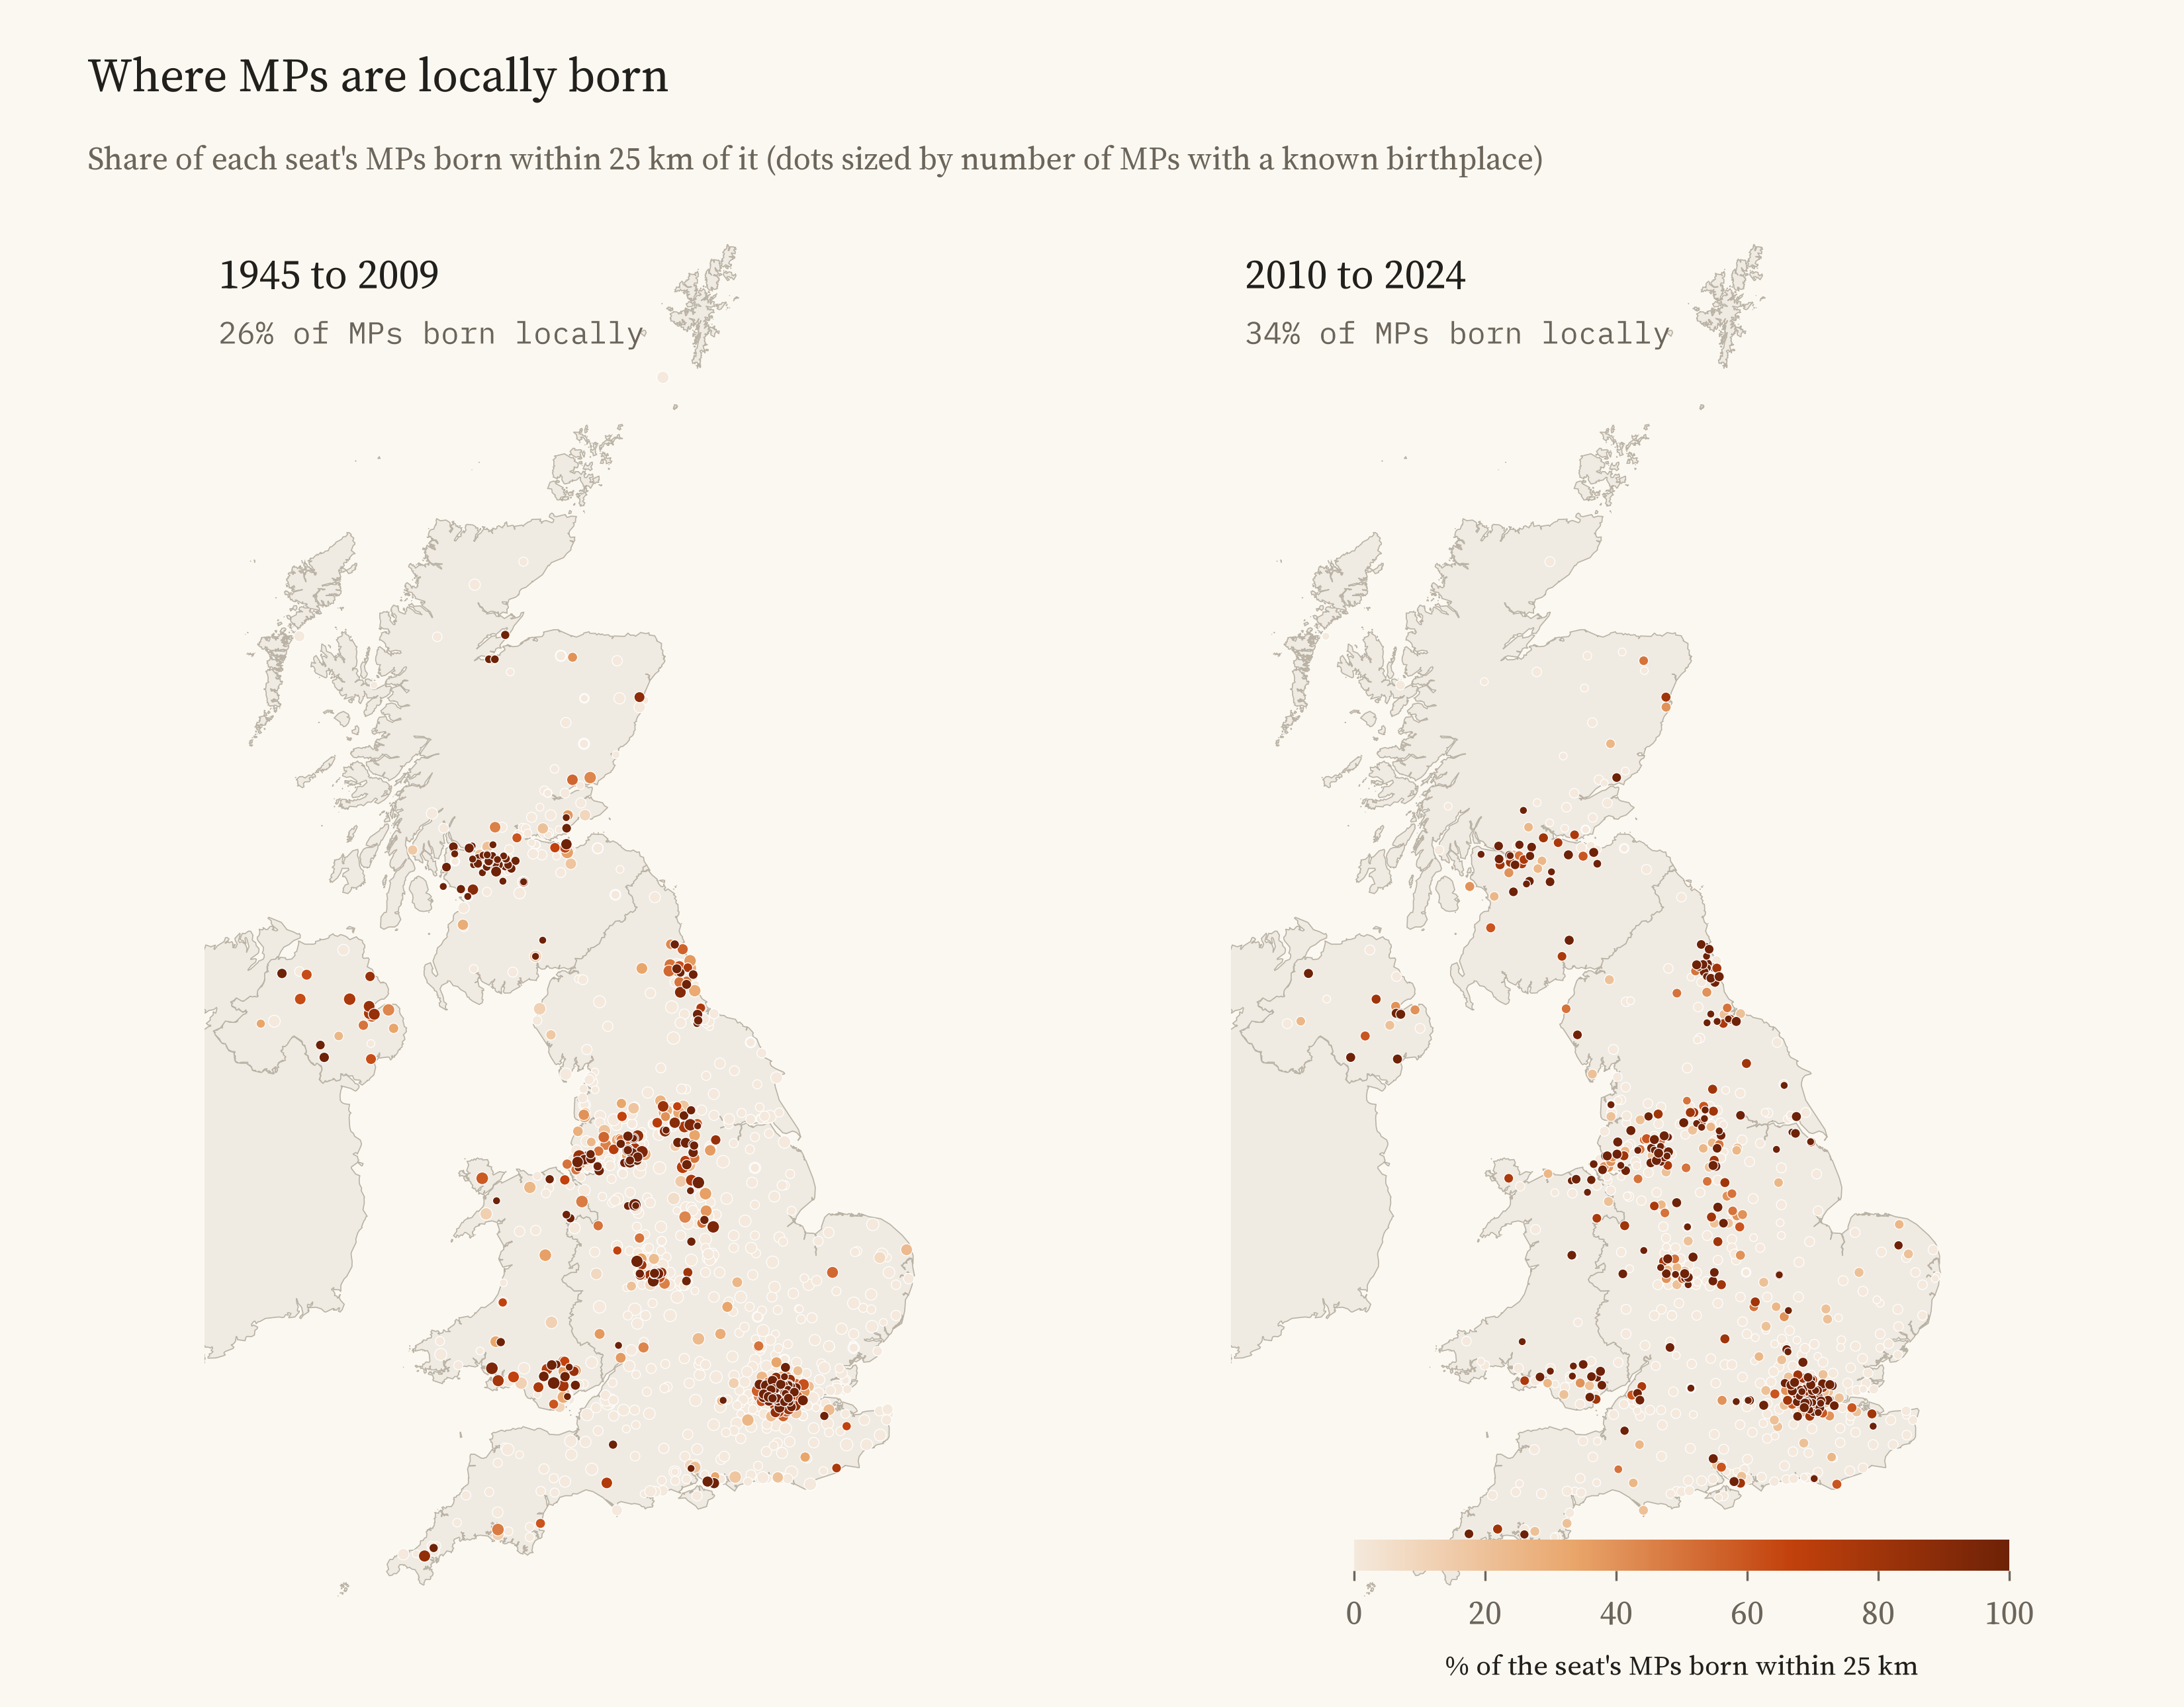
\includegraphics[width=\textwidth]{f_map.png}
\caption{Share of each constituency's MPs born within 25 km of the seat point, 1945 to 2009 and 2010 to 2024 (Great Britain and Northern Ireland; dots sized by the number of MPs with a known birthplace).}\label{fig:map}\end{figure}

\subsection{A local bonus in vote share}
Table~\ref{tab:main} reports the planned main estimates. Local MPs won 1.29 percentage points more of the vote than non-local MPs elected for the same seat, each measured against their party's national performance (95\% CI 0.73 to 1.85; $N=14{,}580$, 1{,}844 constituency clusters). Comparing only MPs of the same party in the same seat (seat by party fixed effects) gives 1.32 (CI 0.70 to 1.95). The raw difference is 1.64 points (55.2\% against 53.5\%), so the fixed effects remove a little of the gap. Measured against the party's national share, the estimate is identical. Without seat fixed effects it is 1.58.

\begin{table}[tbp]\centering\small\caption{Pre-specified main estimates. Vote shares in percentage points.}\label{tab:main}
\begin{tabular}{p{7.4cm}rcrr}\toprule Specification & Estimate & 95\% CI & $p$ & $N$\\\midrule
H1 Vote share (seat FE, election $\times$ party FE) & 1.29 & [0.73, 1.85] & $<$0.001 & 14,580\\
H2 Defeated at next election (LPM, percentage points) & 1.0 & [-0.3, 2.3] & 0.127 & 11,672\\
H3 Change in own share at re-election & 0.31 & [0.06, 0.56] & 0.014 & 10,257\\
H4 Leaving Parliament, Cox hazard ratio & 1.03 & [0.96, 1.10] & 0.374 & 5,042\\
H5 Party share change per step of successor localness & 0.67 & [0.10, 1.24] & 0.021 & 1,138\\
H6 Local $\times$ retires: party share change & -0.86 & [-1.67, -0.06] & 0.035 & 12,494\\
Lead placebo for H5 & 0.17 & [-0.40, 0.74] & 0.559 & 896\\
\bottomrule\end{tabular}\par\vspace{2pt}\parbox{\linewidth}{\footnotesize Standard errors clustered by constituency item unless stated. H2 and H3 control for previous share and tenure with election $\times$ party and nation FE; H4 is stratified by era of first election with party family and nation; H5 and H6 control for previous share with election $\times$ party and nation FE.}\end{table}

How large is a bonus of this size? It is about 16\% of the standard deviation of a party's vote share across seats at the same election (7.9 points in the H1 sample). In terms of voters, it means that in a constituency of 70,000 voters with 65\% turnout, the estimate corresponds to roughly 586 more votes for a local MP than for a non-local one in the same position. It is small next to the swings that national politics produces between elections, which often move a party's national share by several points.

\subsection{No fewer defeats and no longer careers}
Among 11{,}672 incumbents who stood again in a contested contest, 14.5\% were defeated: 14.6\% of local incumbents and 14.5\% of non-local ones. Net of previous share, tenure and fixed effects, the difference is +0.01 (95\% CI -0.00 to +0.02); a logit gives an average marginal effect of +0.00 (CI -0.01 to +0.02). The confidence interval rules out a reduction in defeat probability of more than 0.3 percentage points. Excluding the previous share (exploratory), the estimate is -0.01 (CI -0.02 to +0.01). Local MPs' first unbroken spells lasted 3.04 general elections on average against 3.19; the Cox hazard ratio for leaving is 1.03 (CI 0.96 to 1.10; 5{,}042 MPs, 4{,}590 exits) and for defeat 0.97 (CI 0.87 to 1.09). In the discrete-time model, being local changes the chance of not being returned at the next election by +0.01 (CI -0.01 to +0.02).

The arithmetic explains the contrast. The median winning margin in contested single-member contests since 1832 is 16.6 points; 4.4\% of contests were won by less than the bonus and 9.0\% by less than twice the bonus (since 1945: 7.2\%). A one-point bonus moves the result in only a small share of contests, too few to show in defeat rates with the precision available here.

\subsection{Within-seat changes}
The three designs that exploit changes within seats agree in sign with H1 (Figure~\ref{fig:designs}). Local incumbents gained 0.31 points more at re-election than non-local ones (CI 0.06 to 0.56; $N=10{,}257$). When a seat passed between two MPs of the same party, each step in localness from predecessor to successor raised the party's share relative to its national change by 0.67 points (CI 0.10 to 1.24; $N=1{,}138$ hand-overs); including successors who lost but were MPs at some point gives 0.73 (CI 0.15 to 1.31; $N=1{,}221$). The lead placebo is null: the successor's localness does not predict the party's relative change in the election before the hand-over (0.17, CI -0.40 to 0.74; $N=896$). In the retirement design, when an incumbent stood down the party lost 1.2 points relative to seats where the incumbent stood again, and 0.9 points more when the departing MP was local (interaction -0.86, CI -1.67 to -0.06; $N=12{,}494$).

The succession design deserves a closer look, because it is the one that changes localness while holding the seat and party fixed and comparing elections a single step apart. Of the 1{,}138 hand-overs, 620 were from one non-local MP to another, 158 from one local MP to another, 196 from non-local to local and 164 from local to non-local. Estimated separately against hand-overs with no change, a move from non-local to local raised the party's relative share by 0.85 points (CI -0.02 to 1.73) and a move from local to non-local changed it by -0.47 (CI -1.42 to 0.49). The two effects have opposite signs, as a local bonus implies, the gain somewhat larger than the loss; each alone is imprecise. The lead placebo uses the hand-overs where the outgoing MP had also sat at the previous election in the same seat, so that the party's change in that earlier election is measured with the outgoing MP in place both times; the incoming MP's localness does not predict it.

The retirement design also reproduces the retirement slump familiar from British studies \citep{middleton2019}: whatever the MP's origin, when an incumbent stood down the party's share fell by 1.2 points more than when the incumbent stood again (CI -1.55 to -0.80). The slump was larger for local MPs by 0.9 points. Among MPs who stood again, local MPs' parties also gained 0.36 points more (CI 0.10 to 0.61), which is the H3 estimate in a slightly different sample.

\begin{figure}[tbp]\centering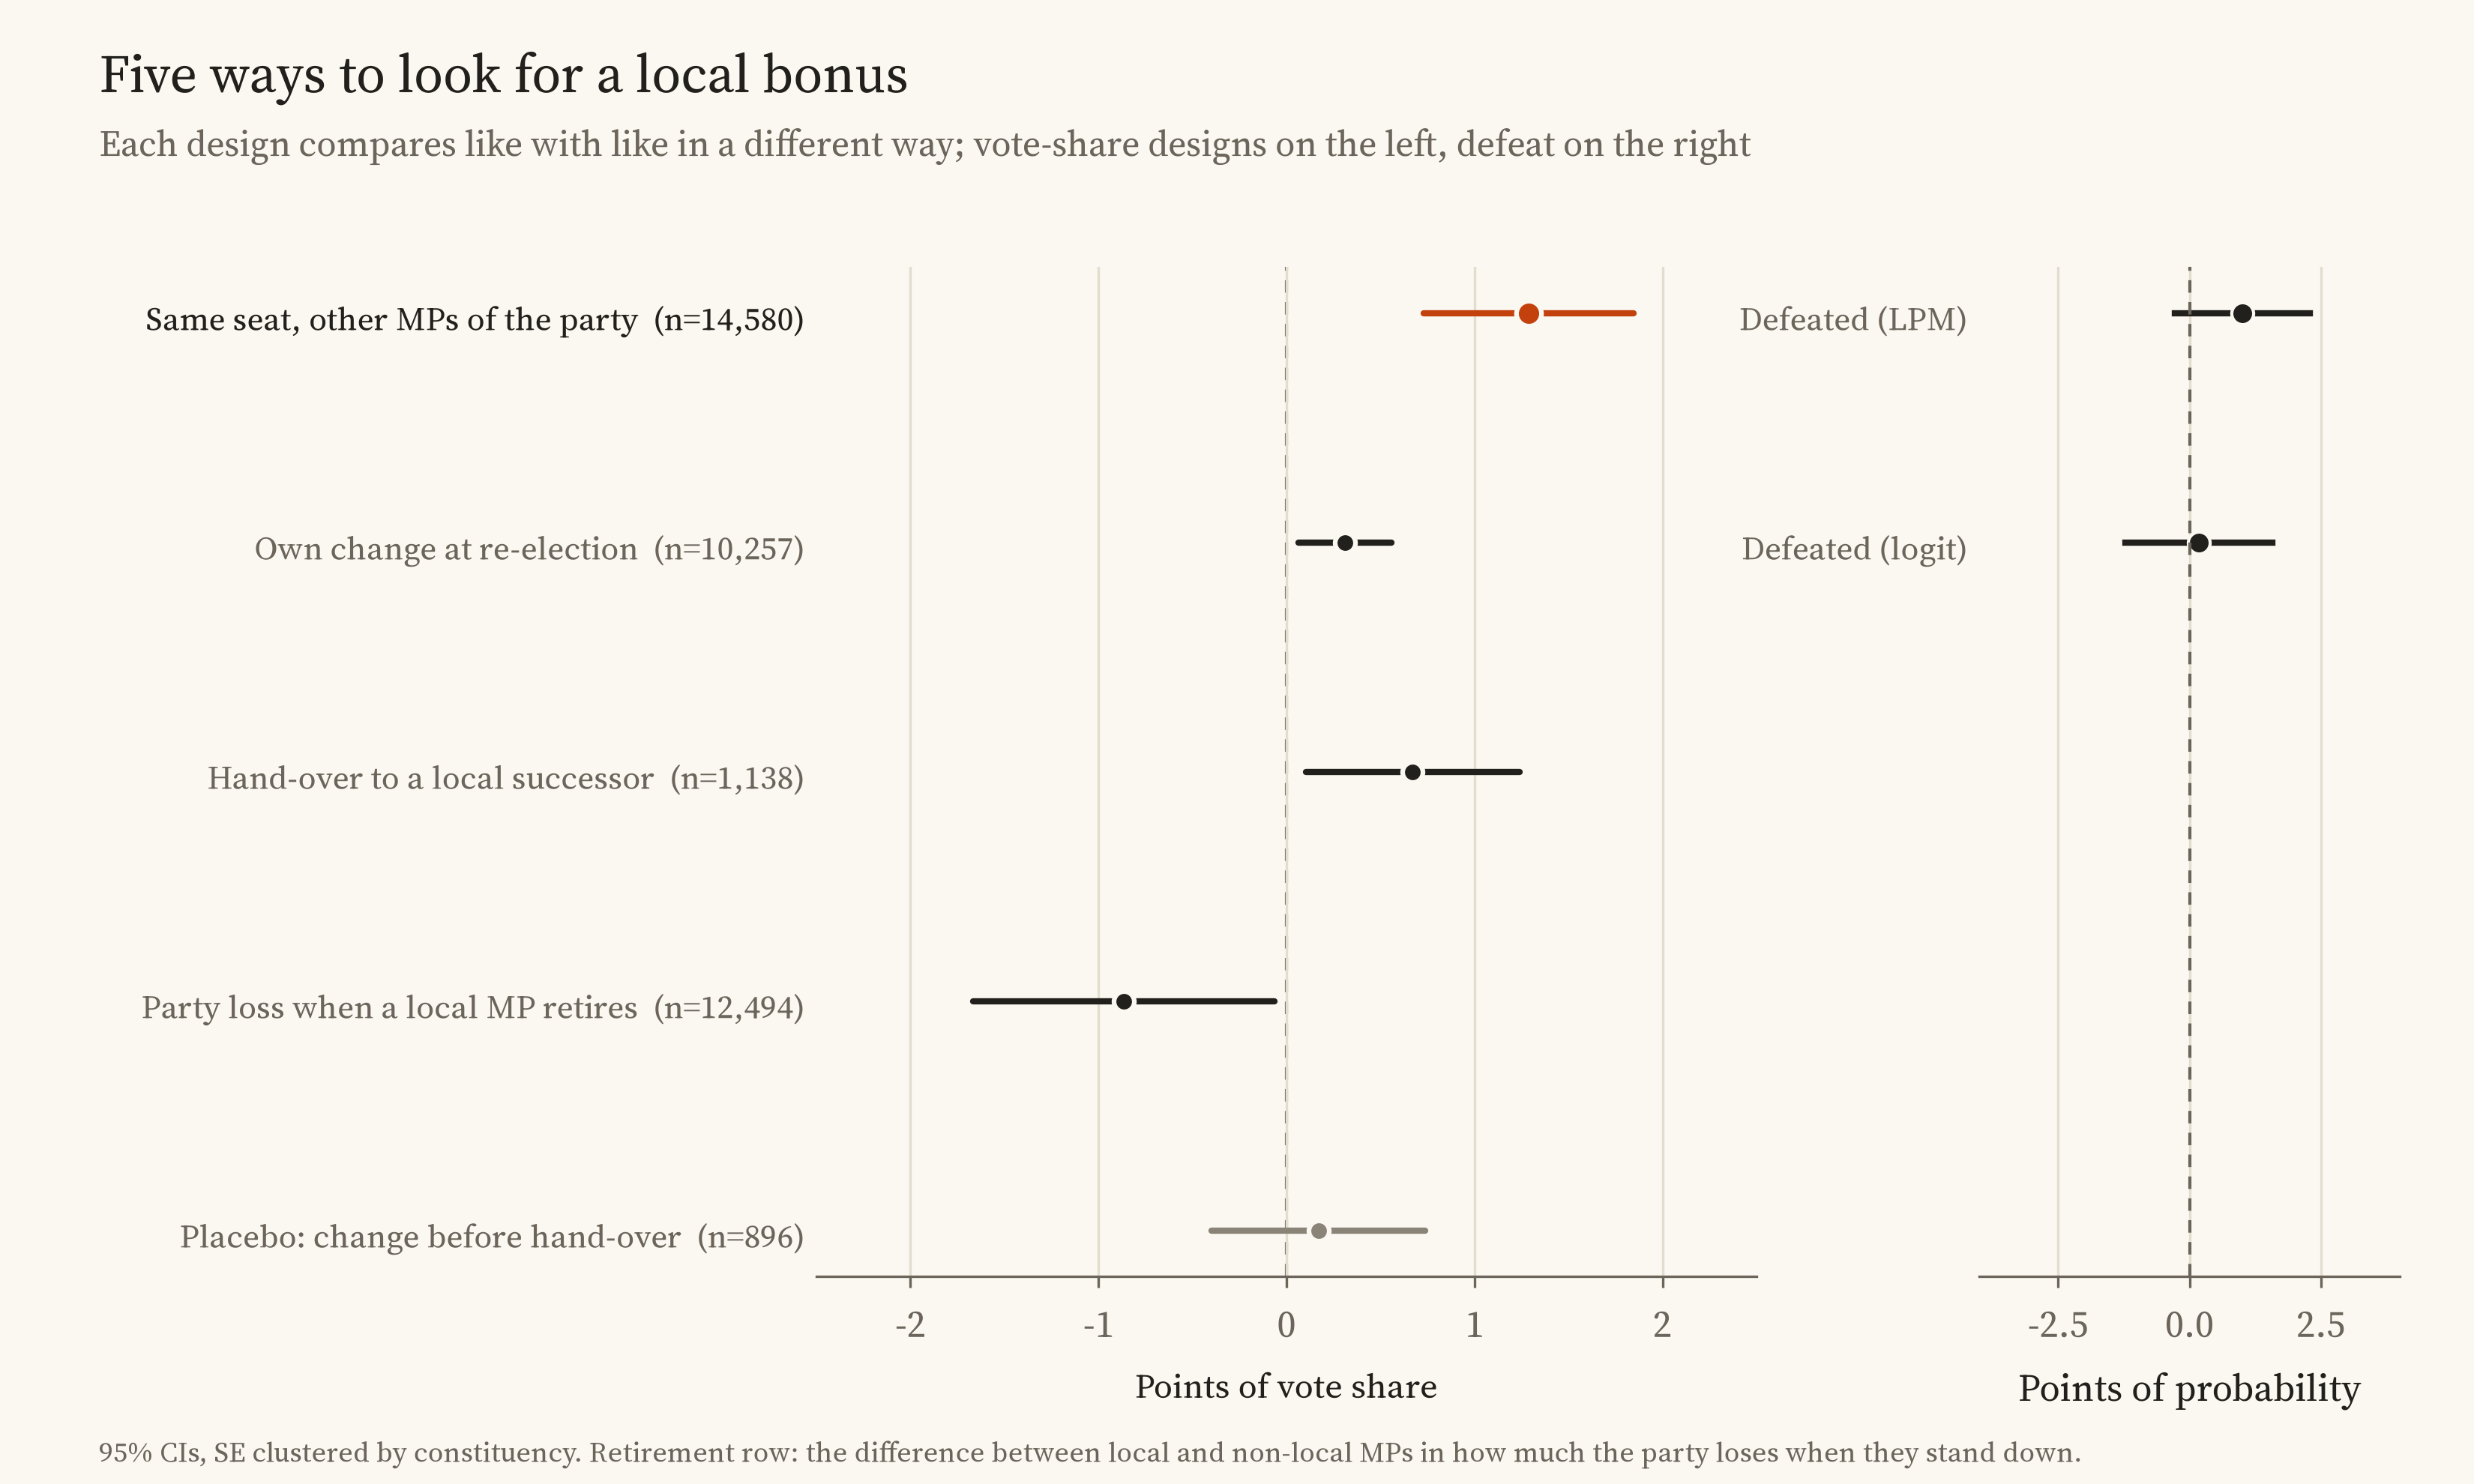
\includegraphics[width=\textwidth]{f_designs.png}
\caption{Estimates from the five designs with 95\% confidence intervals (constituency-clustered). Left: effects on vote share in percentage points; right: effect on the probability of defeat in percentage points.}\label{fig:designs}\end{figure}

\subsection{Heterogeneity}
The level bonus is positive in every era and nation and for the three main party families (Table~\ref{tab:het}, Figure~\ref{fig:groups}). It is 1.60 points from 1832 to 1917, 2.20 from 1918 to 1944, 0.85 from 1945 to 2009 and 0.29 from 2010 to 2024, when the confidence interval (-0.74 to 1.33) includes zero. In England it is 1.12, in Scotland 1.75 and in Wales 2.61. Labour (1.66) and Liberal (2.01) MPs show larger bonuses than Conservatives (0.81, CI -0.10 to 1.73). The differences between groups are mostly within sampling error and were not the object of pre-specified tests of difference, so they should be read as descriptive.

The periods in Figure~\ref{fig:periods} (exploratory) show the same picture at a finer grain. The bonus is imprecisely estimated before 1885, when most seats returned two members and only 360 contested single-member returns with known birthplaces enter the model; it is clearly positive from 1885 to 1935 (1.5 and 2.2 points), smaller and uncertain from 1945 to 1966 (0.2), positive from 1970 to 1992 (1.2) and small since 1997 (0.6 and 0.3). The largest estimates thus come from the period of the Liberal and Labour contest and the widening franchise, when party labels were changing fastest and voters may have relied more on personal cues. The recent rise in localness has not been accompanied by a rise in the bonus. If anything the opposite: the point estimate since 2010 is among the smallest, although its interval is wide and overlaps every other period. A direct test, added at review, of whether the bonus in 2010 to 2024 differs from that in 1832 to 2009 (an interaction of local with the later period, same fixed effects) gives a difference of -1.25 points (CI -2.45 to -0.06, $p=0.040$). This is weak evidence of a smaller recent bonus: it is one of many comparisons, it was not planned, and the upper end of the interval is close to zero.

Across nations, the Welsh estimate is the largest and the English the smallest of the three British nations, but the intervals overlap widely. The Conservative estimate is smaller than Labour's and the Liberals', and its interval includes zero. One possible reading is that Conservative voters weigh party and leadership more and local roots less, another that Conservative MPs who are local in the birthplace sense are less often local in the sense voters notice; the data cannot distinguish these.

\begin{figure}[tbp]\centering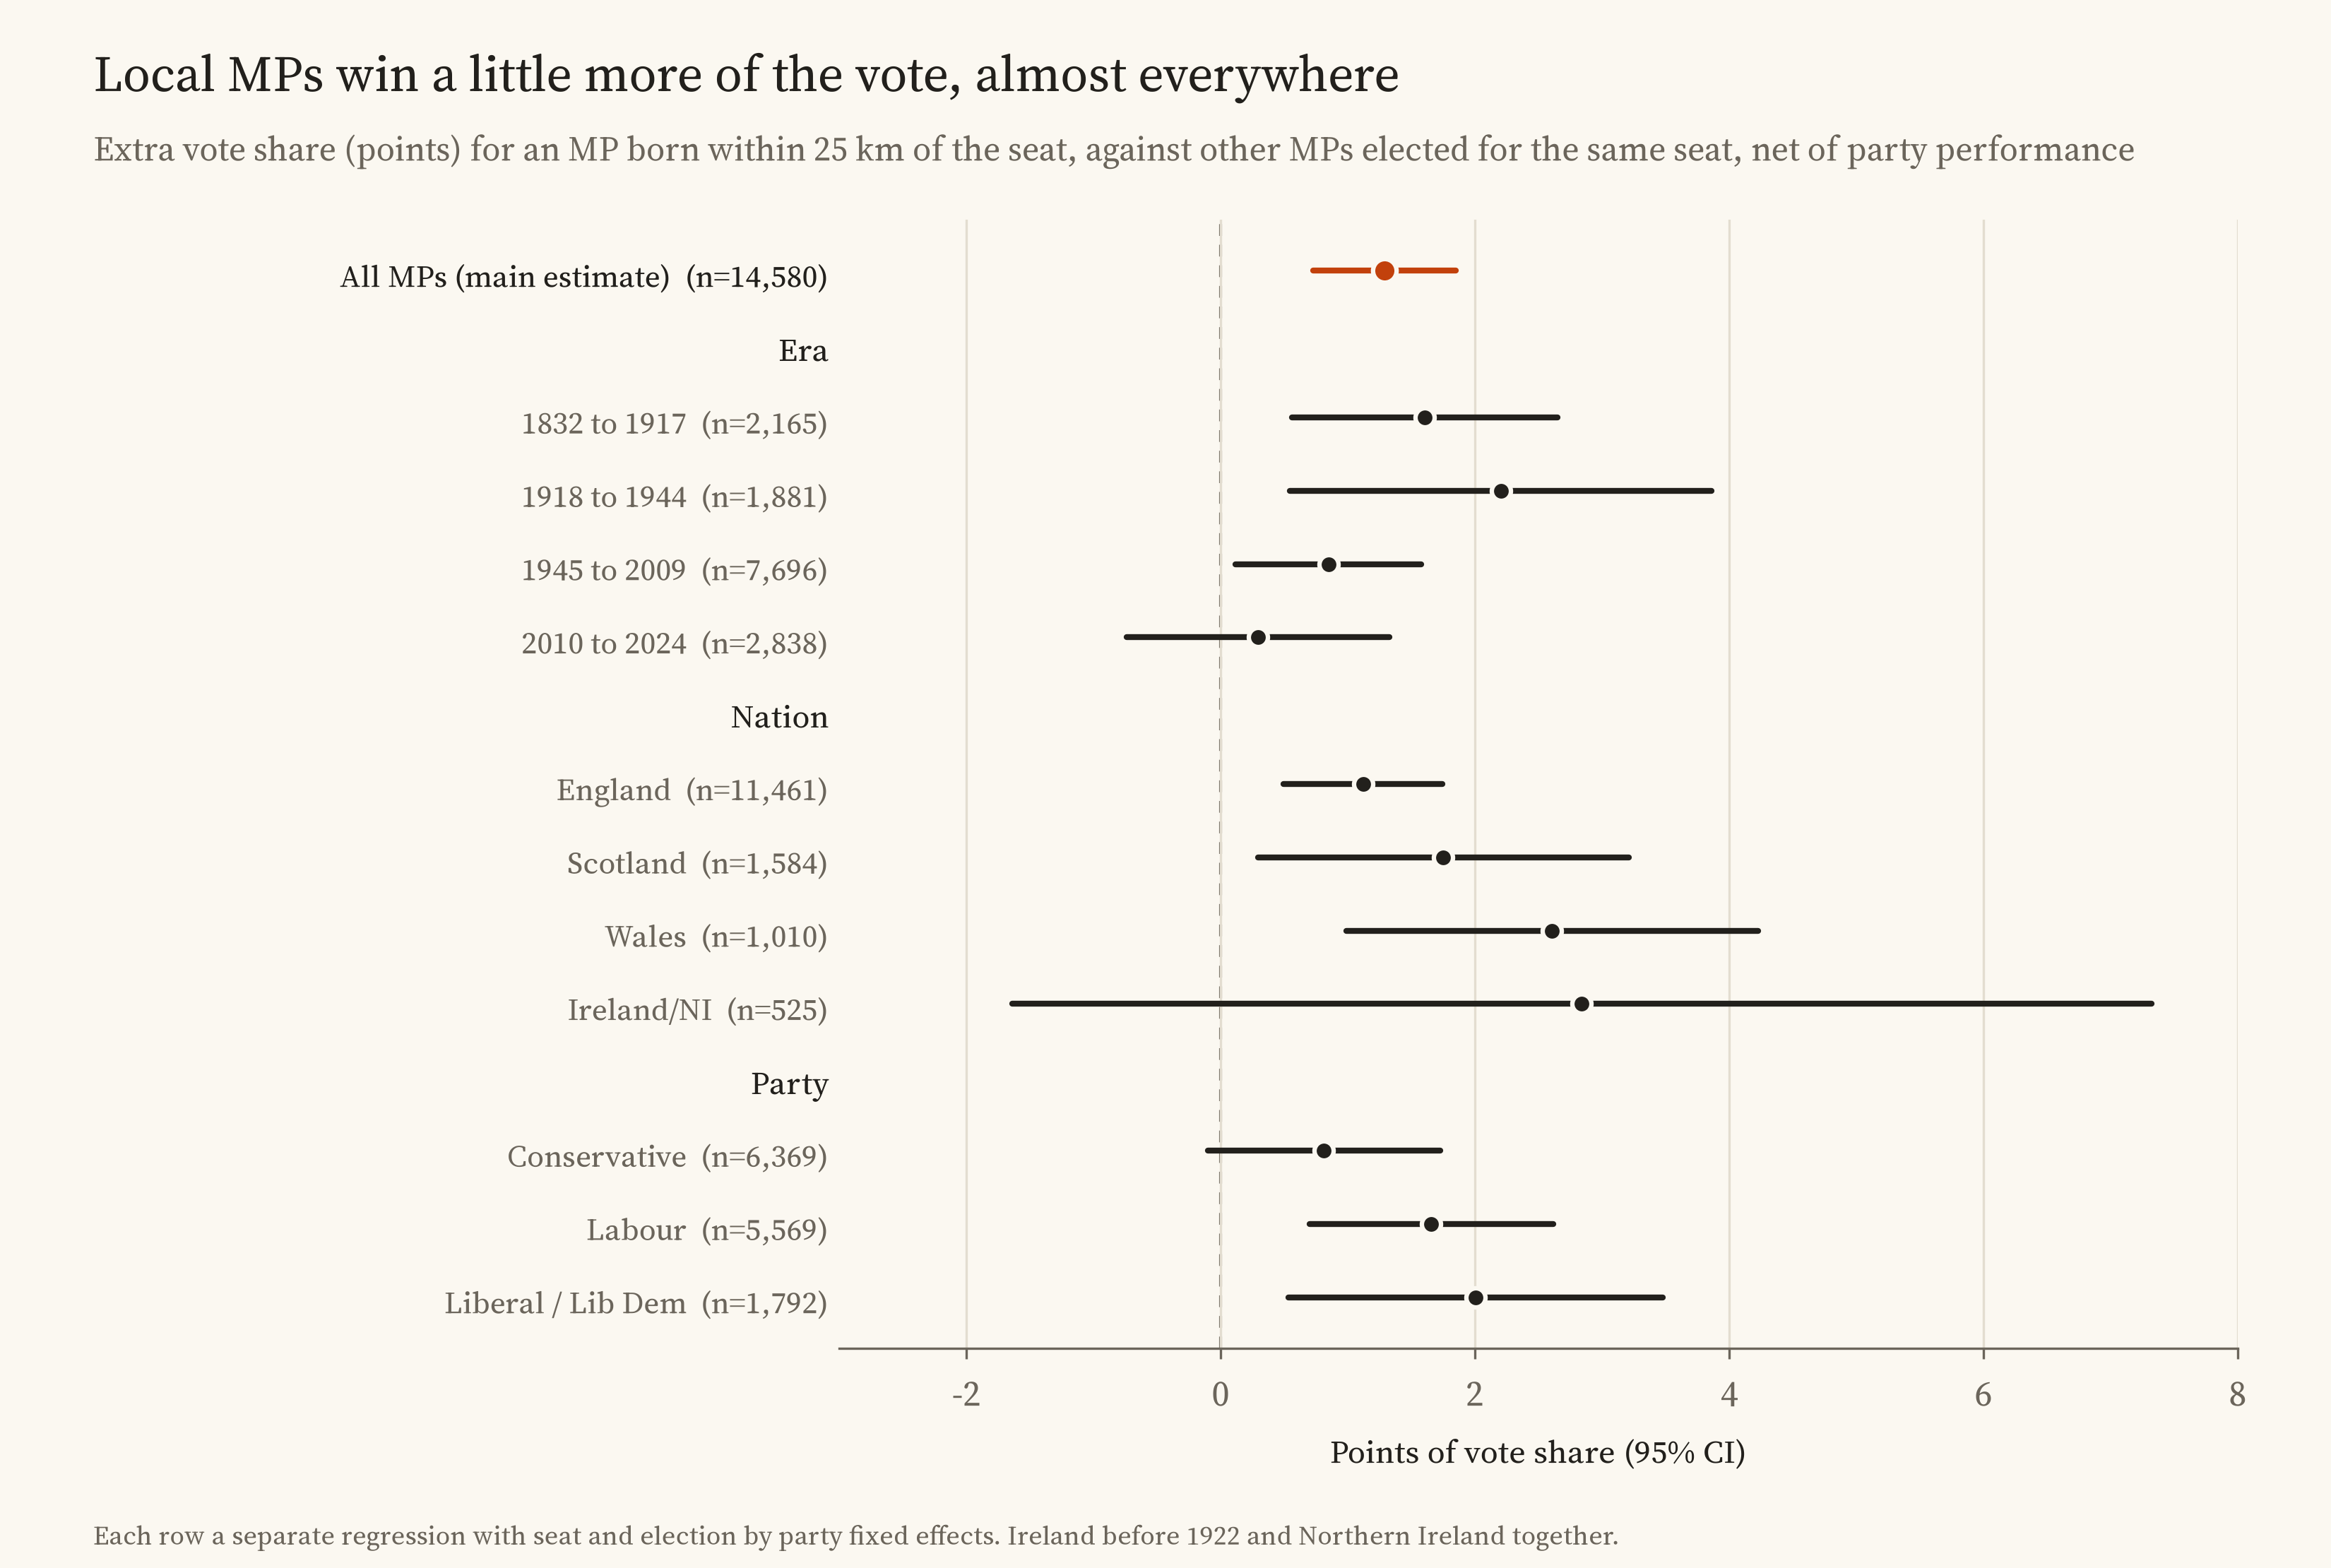
\includegraphics[width=0.95\textwidth]{f_groups.png}
\caption{The level bonus (H1) by era, nation and party family; separate regressions with seat and election by party fixed effects.}\label{fig:groups}\end{figure}

\begin{table}[tbp]\centering\small\caption{Heterogeneity: separate regressions by era, nation and party family (estimate and 95\% CI).}\label{tab:het}
\begin{tabular}{lccc}\toprule Group & H1 share & H2 defeat (pp) & H3 change\\\midrule
1832 to 1917 & 1.60 [0.56, 2.65] & -1.7 [-5.2, 1.8] & 0.45 [-0.44, 1.34]\\
1918 to 1944 & 2.20 [0.54, 3.86] & 2.7 [-1.5, 7.0] & 0.24 [-0.80, 1.28]\\
1945 to 2009 & 0.85 [0.12, 1.58] & 0.2 [-1.2, 1.5] & 0.47 [0.23, 0.71]\\
2010 to 2024 & 0.29 [-0.74, 1.33] & 3.0 [-0.4, 6.4] & -0.25 [-0.88, 0.39]\\
\midrule
England & 1.12 [0.50, 1.75] & 0.5 [-0.9, 1.9] & \\
Scotland & 1.75 [0.30, 3.21] & 1.1 [-2.8, 5.1] & \\
Wales & 2.61 [0.99, 4.23] & -0.4 [-4.9, 4.1] & \\
Ireland/NI & 2.84 [-1.64, 7.32] & 4.6 [-2.0, 11.1] & \\
\midrule
Conservative & 0.81 [-0.10, 1.73] & 2.4 [0.3, 4.5] & -0.07 [-0.45, 0.31]\\
Labour & 1.66 [0.70, 2.62] & 0.4 [-1.3, 2.1] & 0.52 [0.18, 0.85]\\
Liberal / Lib Dem & 2.01 [0.53, 3.48] & -2.9 [-6.7, 1.0] & 0.14 [-0.94, 1.22]\\
\bottomrule\end{tabular}\par\vspace{2pt}\parbox{\linewidth}{\footnotesize Standard errors clustered by constituency item unless stated. Ns in the replication files (data/models.json).}\end{table}

\begin{figure}[tbp]\centering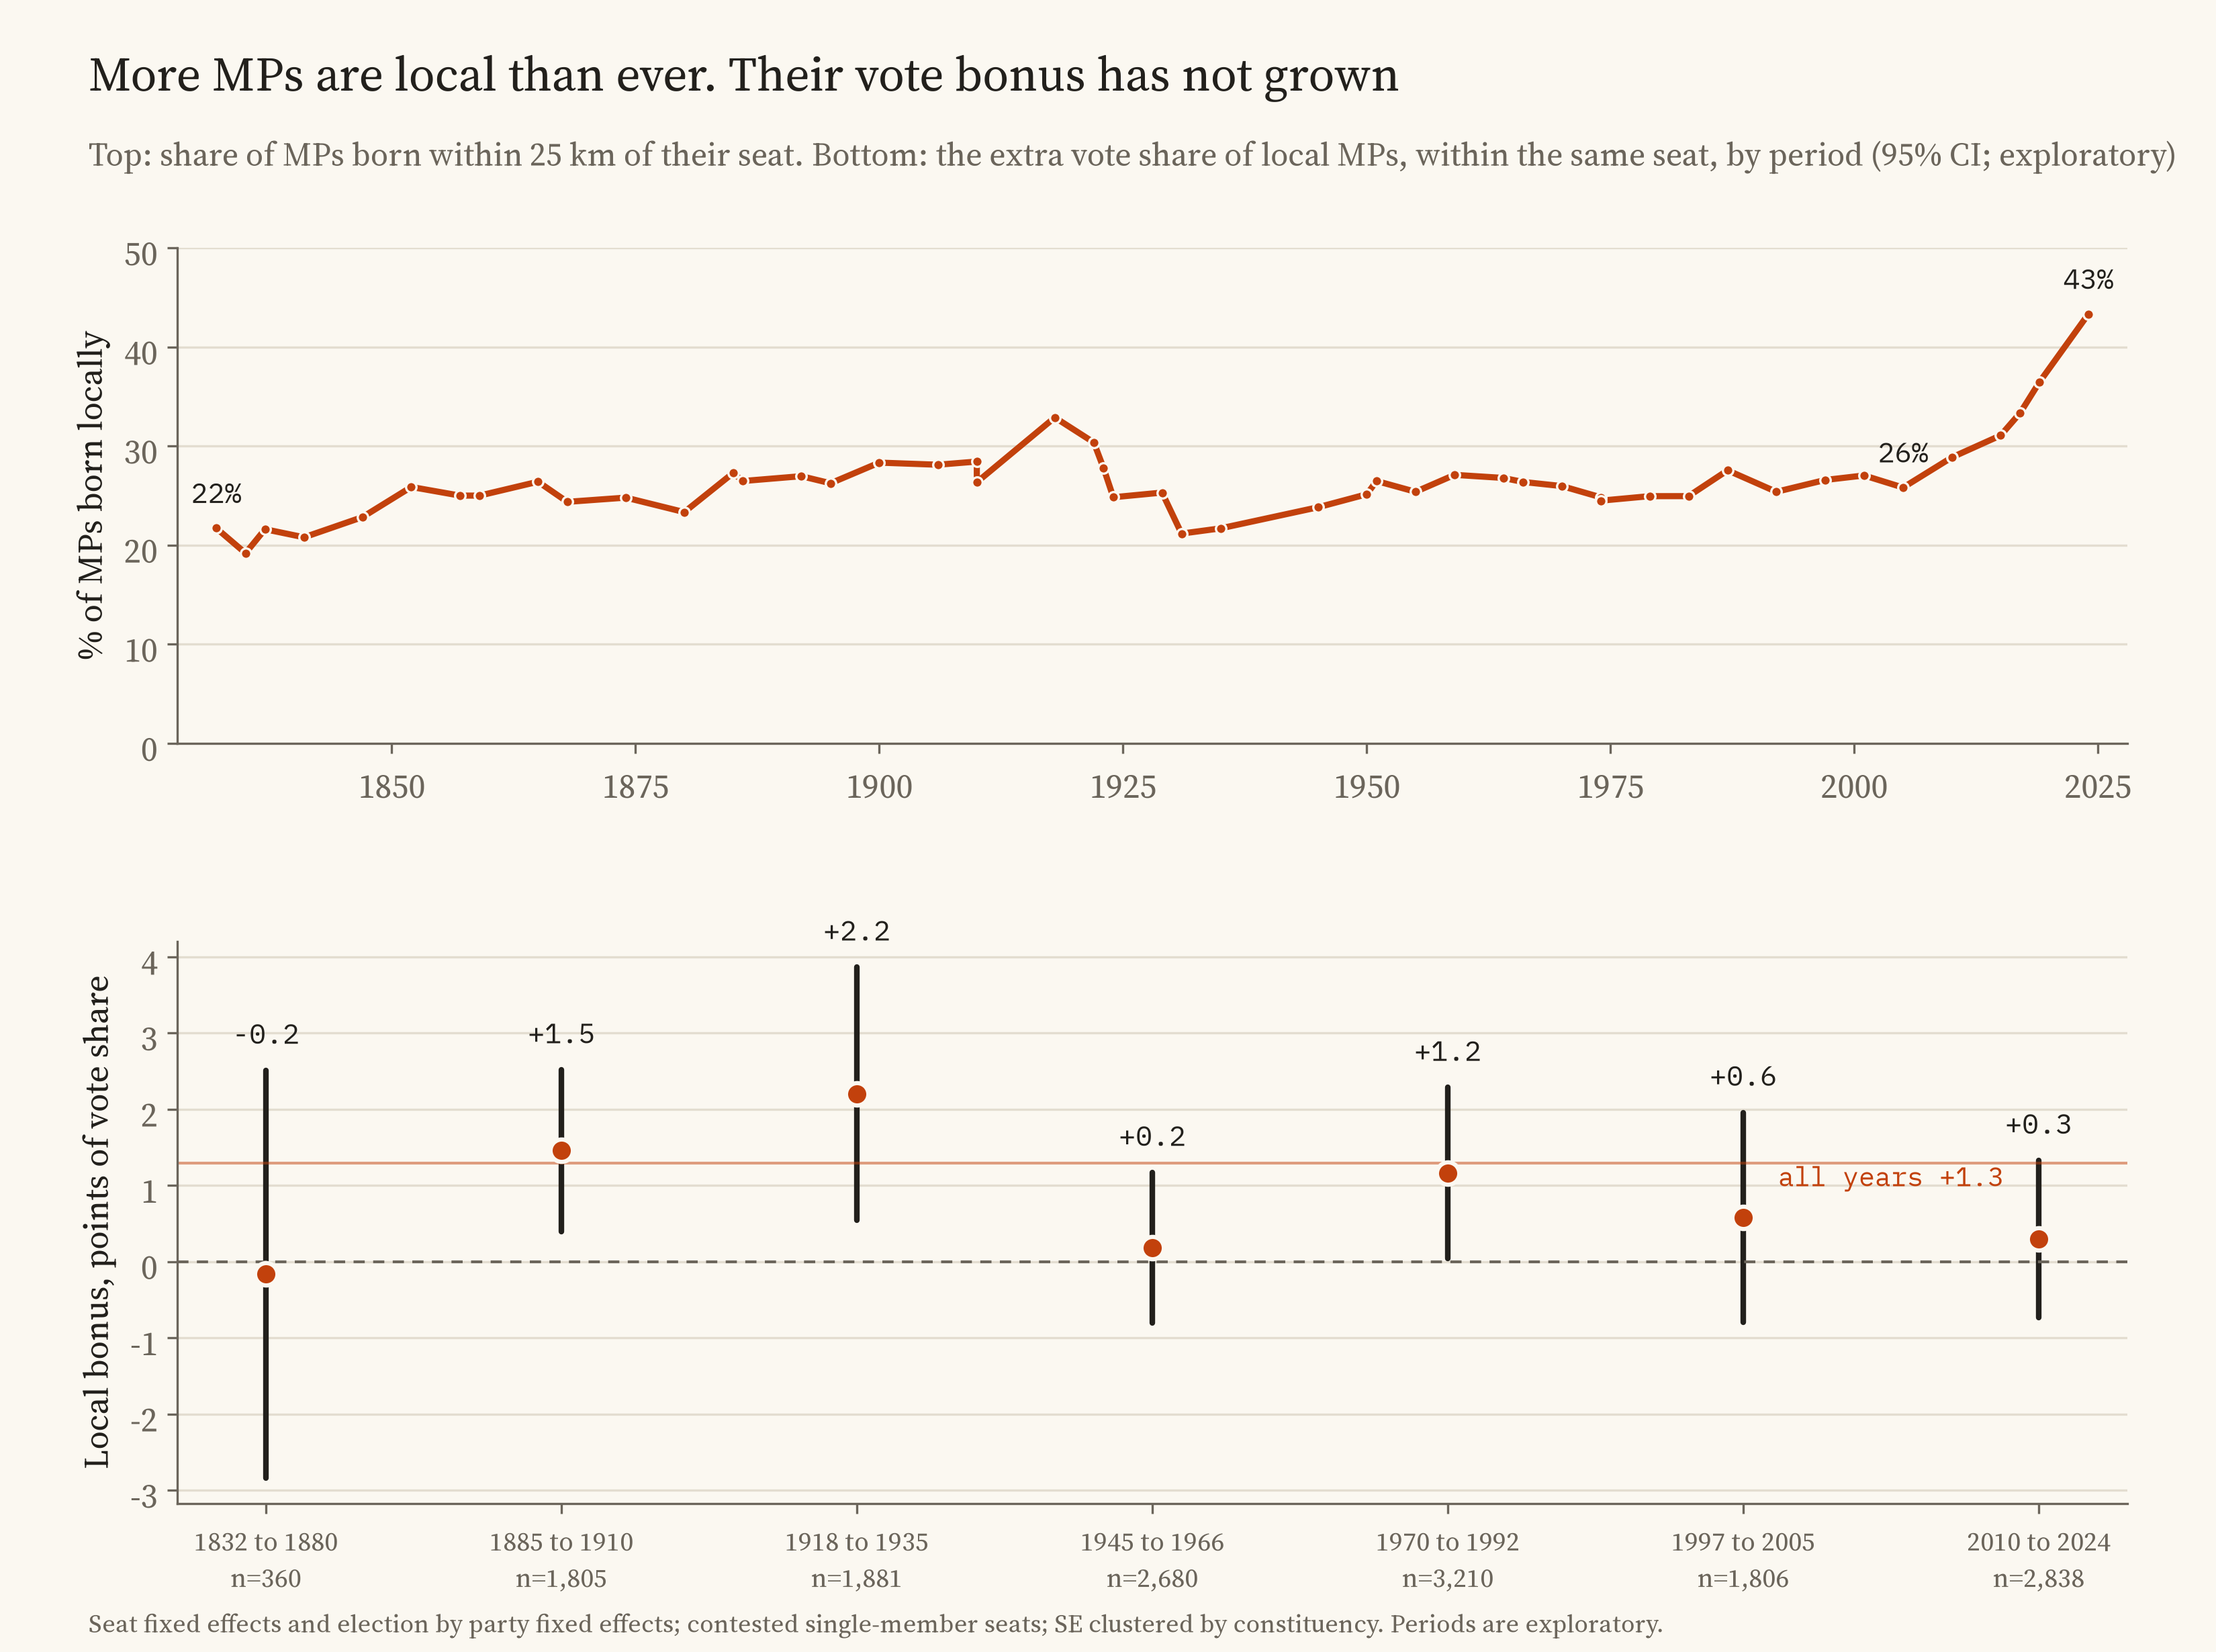
\includegraphics[width=0.95\textwidth]{f_periods.png}
\caption{Top: share of MPs with a known birthplace born within 25 km of their seat, by general election (elections with at least 40 placed MPs). Bottom: the H1 bonus by period (exploratory splits), 95\% CIs.}\label{fig:periods}\end{figure}

\section{Robustness}
The main estimate is stable across specifications and measurement choices (Table~\ref{tab:rob}, Figure~\ref{fig:robust}), ranging from 0.93 to 1.51 across alternative fixed effects, clustering and definitions, and from 1.07 to 2.05 when each nation or era is left out. Every alternative excludes zero. The advantage is concentrated close to the seat: being born 0 to 25 km away adds 1.23 points relative to over 100 km, while 25 to 100 km is indistinguishable from over 100 km (-0.18, CI -0.70 to 0.33), and in the continuous version each doubling of $1+$distance lowers the share by 0.19 points. Keeping MPs with unknown birthplaces as a separate category gives 1.14, so the result does not depend on dropping them; the unknown category itself differs from non-local MPs by -0.54 points (CI -0.88 to -0.20), consistent with their being on average less prominent members, and giving no sign that a large group of local MPs is hidden among them.

\textbf{Measurement.} The gradient by distance is informative about mechanisms as well as robustness. The effect at 10 km (1.22) is similar to that at 25 km, and the 50 km version is smaller (0.98), because it adds MPs born at a distance where any local advantage is weaker. Using the county instead of a radius gives 0.93: counties are coarse, and county seats are placed at points that can be far from parts of the county. Restricting to seats placed at their own coordinates, which removes the roughest seat points, gives 1.35, and restricting to birthplaces from Wikidata gives 1.51; both suggest that measurement error in the main sample, if anything, attenuates the estimate.

\begin{figure}[tbp]\centering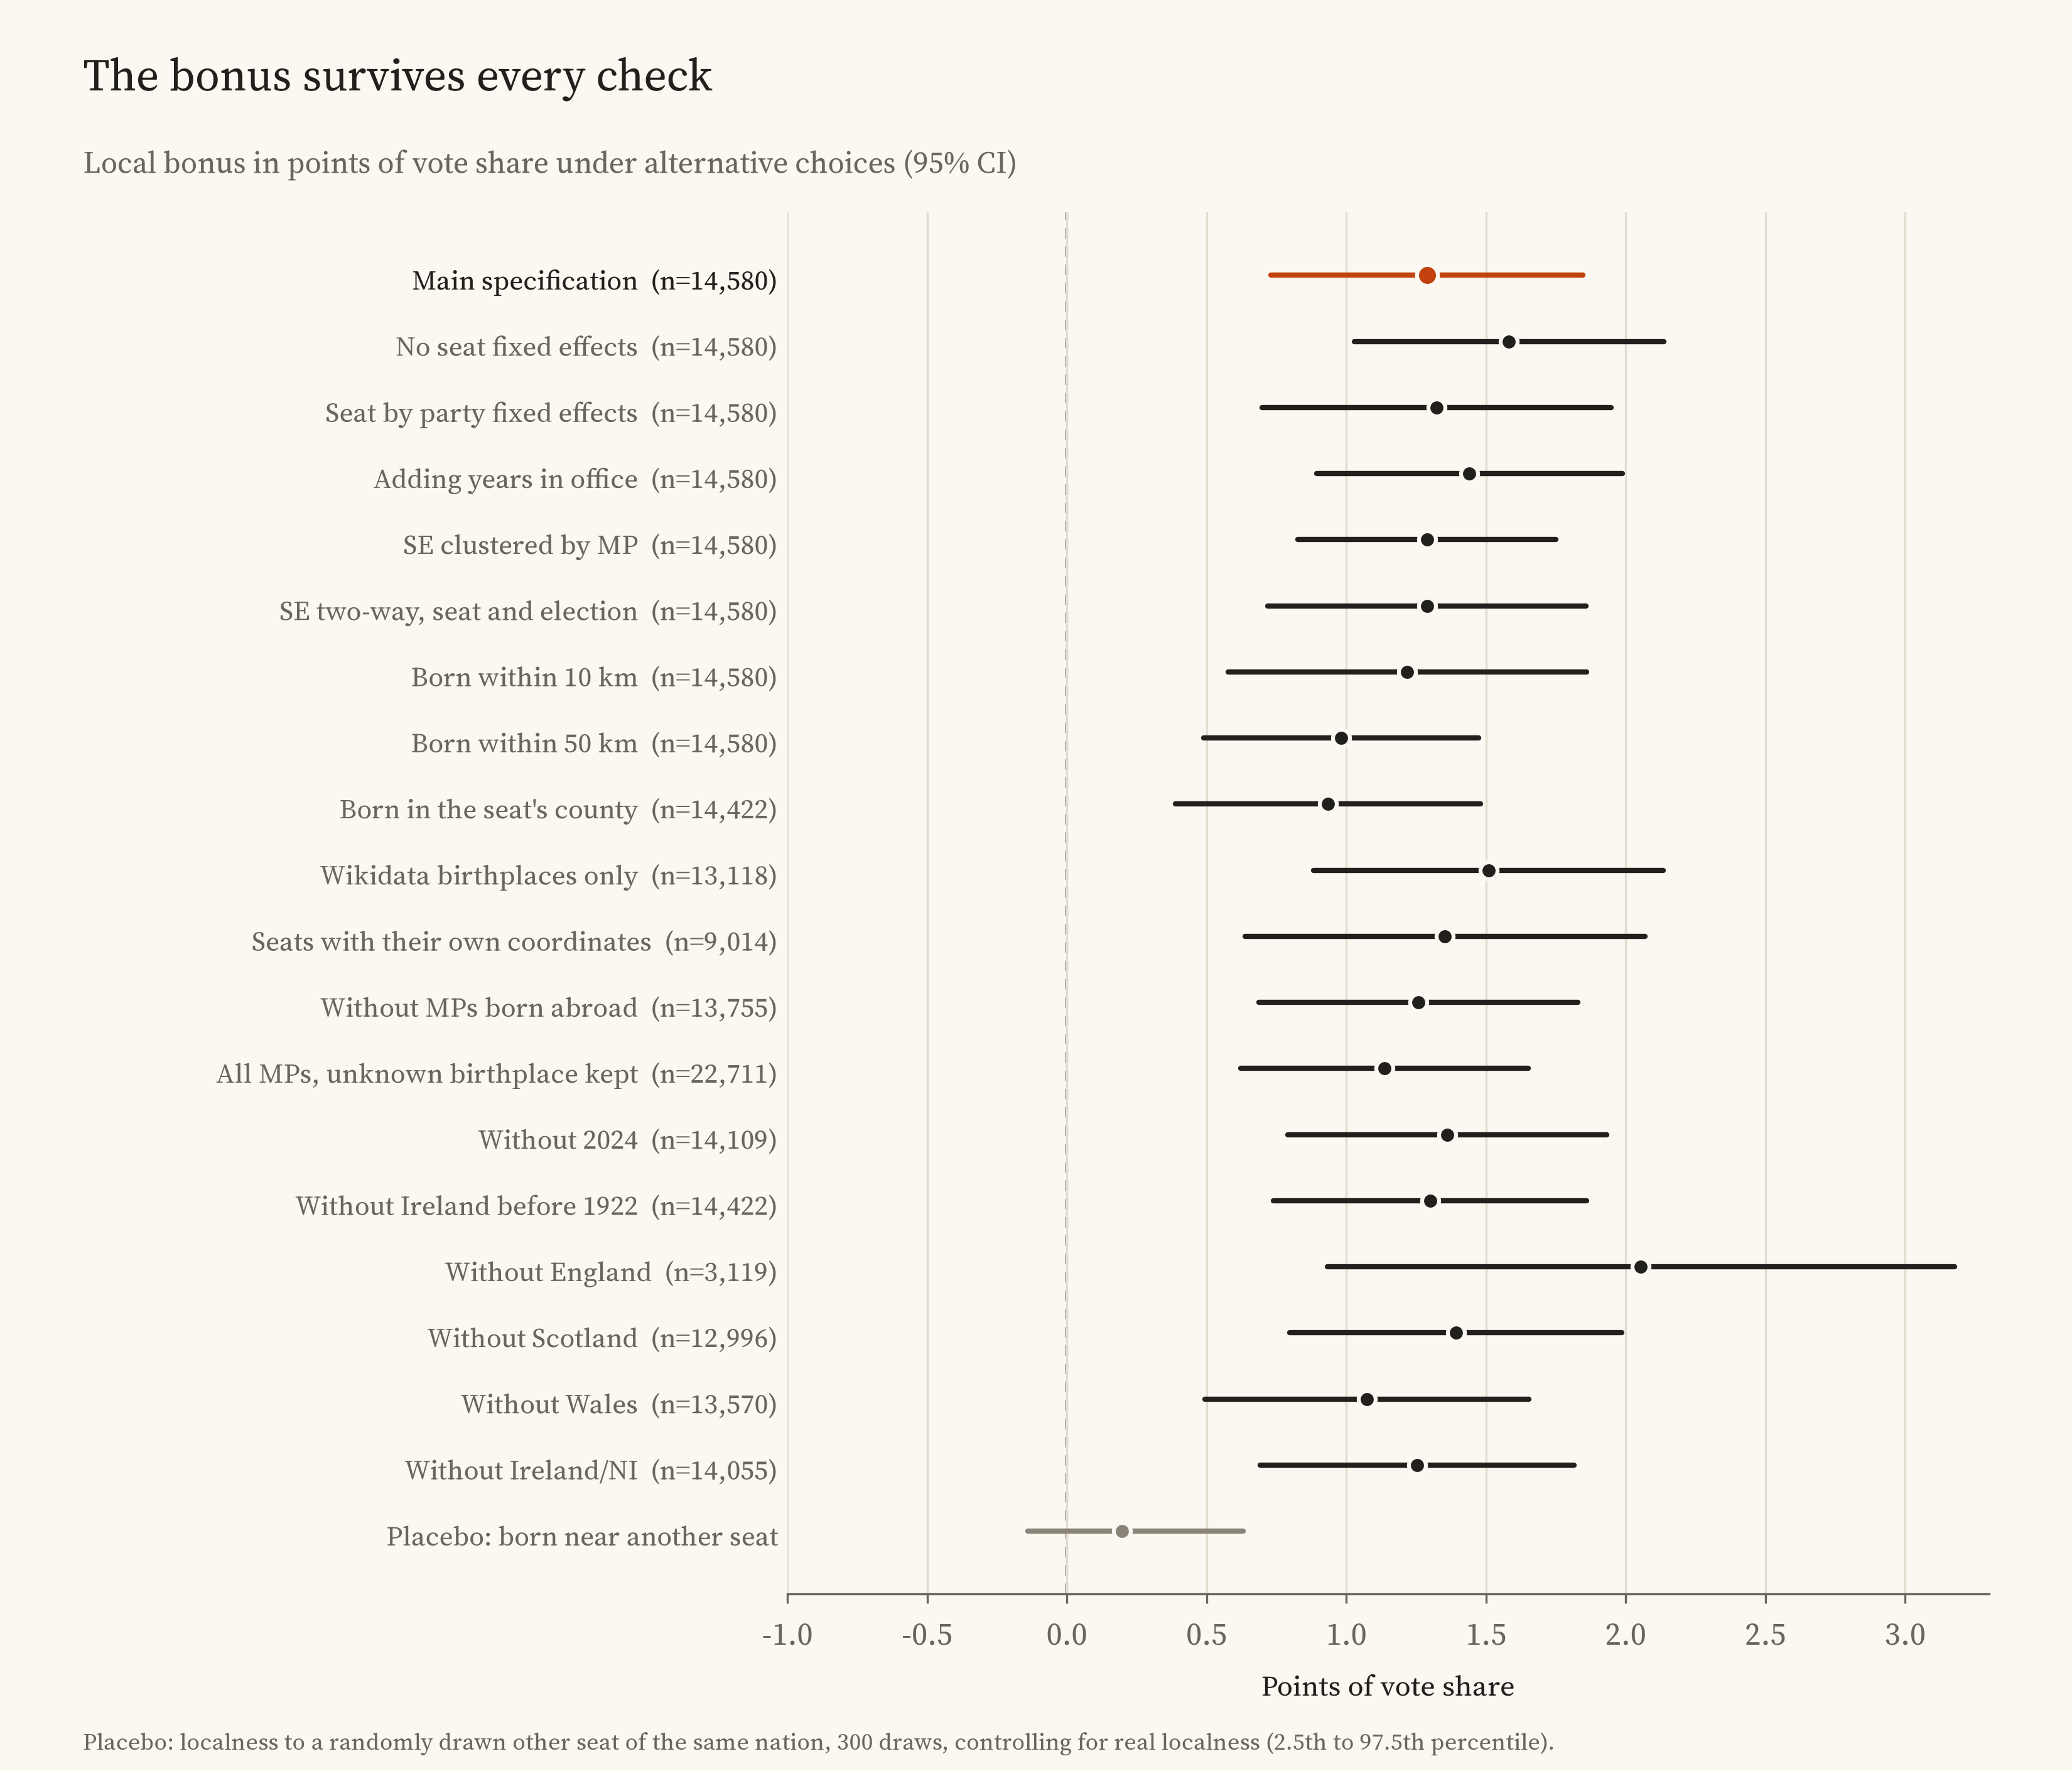
\includegraphics[width=0.95\textwidth]{f_robust.png}
\caption{The H1 bonus under alternative specifications and samples, with the conditional fake-seat placebo (grey).}\label{fig:robust}\end{figure}

\begin{table}[tbp]\centering\small\caption{Robustness of the level bonus (H1). Percentage points of vote share.}\label{tab:rob}
\begin{tabular}{p{7.4cm}rcrr}\toprule Specification & Estimate & 95\% CI & $p$ & $N$\\\midrule
Main & 1.29 & [0.73, 1.85] & $<$0.001 & 14,580\\
Outcome: share minus party national share & 1.29 & [0.73, 1.85] & $<$0.001 & 14,580\\
No seat FE (nation FE) & 1.58 & [1.03, 2.14] & $<$0.001 & 14,580\\
Seat $\times$ party FE & 1.32 & [0.70, 1.95] & $<$0.001 & 14,580\\
Adding tenure & 1.44 & [0.89, 1.99] & $<$0.001 & 14,580\\
SE clustered by MP & 1.29 & [0.83, 1.75] & $<$0.001 & 14,580\\
SE two-way: seat and election & 1.29 & [0.72, 1.86] & $<$0.001 & 14,580\\
Local = within 10 km & 1.22 & [0.58, 1.86] & $<$0.001 & 14,580\\
Local = within 50 km & 0.98 & [0.49, 1.47] & $<$0.001 & 14,580\\
Local = born in seat's county & 0.93 & [0.39, 1.48] & $<$0.001 & 14,422\\
log(1 + km), per unit & -0.27 & [-0.39, -0.15] & $<$0.001 & 14,580\\
Wikidata birthplaces only & 1.51 & [0.88, 2.13] & $<$0.001 & 13,118\\
Seats with own coordinates only & 1.35 & [0.64, 2.07] & $<$0.001 & 9,014\\
Excluding MPs born abroad & 1.26 & [0.69, 1.83] & $<$0.001 & 13,755\\
Unknown birthplace kept as a category & 1.14 & [0.62, 1.65] & $<$0.001 & 22,711\\
Without 2024 & 1.36 & [0.79, 1.93] & $<$0.001 & 14,109\\
Without Ireland before 1922 & 1.30 & [0.74, 1.86] & $<$0.001 & 14,422\\
Without England & 2.05 & [0.93, 3.18] & $<$0.001 & 3,119\\
Without Scotland & 1.39 & [0.80, 1.99] & $<$0.001 & 12,996\\
Without Wales & 1.07 & [0.49, 1.65] & $<$0.001 & 13,570\\
Without Ireland/NI & 1.25 & [0.69, 1.82] & $<$0.001 & 14,055\\
Without 1832 to 1917 & 1.24 & [0.61, 1.87] & $<$0.001 & 12,415\\
Without 1918 to 1944 & 1.17 & [0.57, 1.76] & $<$0.001 & 12,699\\
Without 1945 to 2009 & 1.07 & [0.32, 1.82] & 0.005 & 6,884\\
Without 2010 to 2024 & 1.32 & [0.72, 1.93] & $<$0.001 & 11,742\\
Bands: 0 to 25 km (ref. over 100) & 1.23 & [0.65, 1.81] & $<$0.001 & 14,580\\
Bands: 25 to 100 km & -0.18 & [-0.70, 0.33] & 0.479 & \\
Candidacies of ever-MPs, winners and losers & 3.76 & [3.02, 4.50] & $<$0.001 & 20,981\\
\midrule
\multicolumn{5}{l}{\emph{Added at review (exploratory)}}\\
First-time winners only & 1.31 & [0.66, 1.95] & $<$0.001 & 3,989\\
Seat $\times$ party FE, adding tenure & 1.45 & [0.83, 2.07] & $<$0.001 & 14,580\\
First-time winners, lagged party seat strength & 1.18 & [0.55, 1.81] & $<$0.001 & 3,259\\
All returns, lagged party seat strength and tenure & 1.12 & [0.69, 1.55] & $<$0.001 & 12,908\\
Local $\times$ 2010 to 2024 (difference from 1832 to 2009) & -1.25 & [-2.45, -0.06] & 0.040 & 14,580\\
\bottomrule\end{tabular}\par\vspace{2pt}\parbox{\linewidth}{\footnotesize Standard errors clustered by constituency item unless stated.}\end{table}

\textbf{Placebos.} Permuting localness within election by party cells gives coefficients centred on 0.008 (standard deviation 0.127); none of 500 permutations reached the real estimate (permutation $p<0.002$). Being born within 25 km of a randomly chosen other seat of the same nation has a small positive coefficient on its own (0.27, 95\% of draws between -0.06 and 0.70), because the random seat is sometimes near the MP's own; the two further versions below were added after this first run and are a labelled deviation from the plan (Appendix). Restricted to seats at least 50 km away it is -0.11 (-0.59 to 0.44), and with real localness in the model it is 0.20 (-0.14 to 0.63) while the real coefficient is unchanged. The small positive mean of the conditional version comes from random seats that lie close to the MP's own seat, where being born nearby is a weaker form of localness; for random seats at least 50 km away the placebo is centred below zero. Figure~\ref{fig:placebo} summarises.

\begin{figure}[tbp]\centering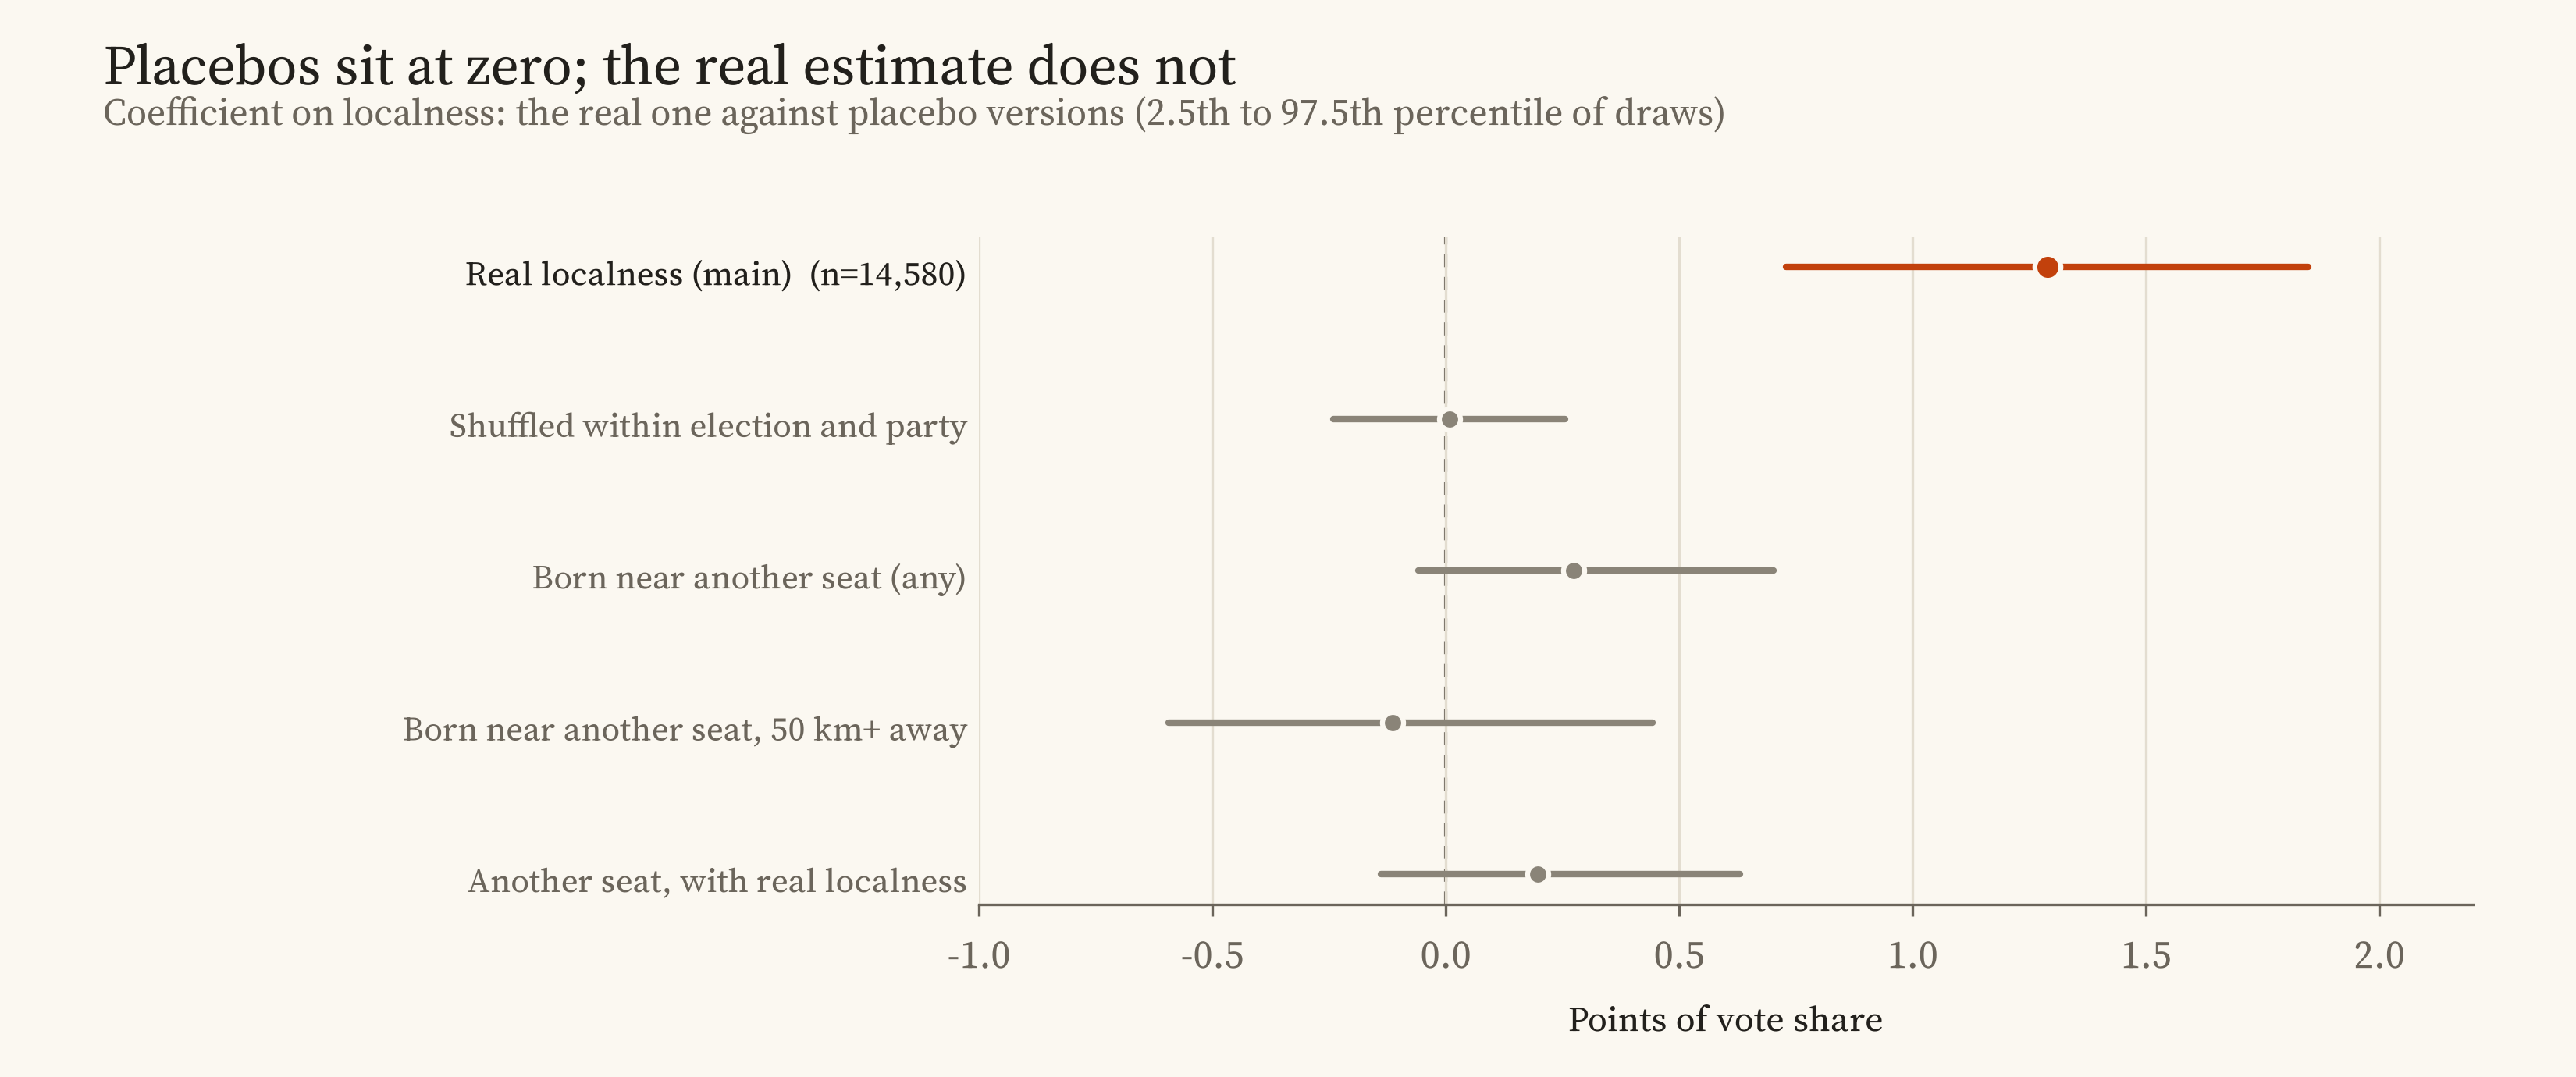
\includegraphics[width=0.95\textwidth]{f_placebo.png}
\caption{Real localness against placebo versions: permuted within election by party (mean $\pm$1.96 SD of draws) and localness to random other seats (2.5th to 97.5th percentiles of draws).}\label{fig:placebo}\end{figure}

\textbf{Boundaries.} Constituency items persist across many redistributions, so some ``same seat'' comparisons span boundary changes. Excluding election pairs that span a general redistribution, the re-election estimate (H3) falls to 0.16 (CI -0.14 to 0.46) while the retirement interaction (H6) strengthens to -1.22 (CI -2.09 to -0.34); the defeat estimate is unchanged (+0.01). With seat fixed effects in place of nation fixed effects, H3 is 0.63 and H6 -0.86. H3 is the least robust of the vote-share designs: with same-county localness it is 0.20 (CI -0.05 to 0.45) and at first re-elections alone 0.18 (CI -0.28 to 0.64).

\textbf{Candidate-level check.} Pooling all candidacies of people who were MPs at some point, winners and losers (20{,}981 candidacies, 6{,}384 losing), with seat and election by party fixed effects, local candidates won 3.76 points more (CI 3.02 to 4.50) and were 9.1 percentage points more likely to win. This larger estimate mixes the local bonus with selection, since ever-MPs who stood far from home and lost are often candidates fielded in unwinnable seats, and is not used as evidence for H1.

\textbf{Checks added at review (exploratory).} Four further checks address incumbency and selection; they were added after the planned results were known. First, among first-time winners only, who have no accumulated incumbency, the bonus is 1.31 (CI 0.66 to 1.95; $N=3{,}989$), and with seat by party fixed effects and tenure it is 1.45 (CI 0.83 to 2.07). Second, a balance test: among first-time winners, the party's own share in the seat at the previous general election, relative to its national share, does not predict whether the new MP is local (a 10-point stronger party changes the probability of a local MP by 0.001, CI per point -0.002 to 0.002; $N=3{,}259$). Third, controlling for that lagged party strength the bonus is 1.18 among first-time winners (CI 0.55 to 1.81) and 1.12 among all returns with tenure also controlled (CI 0.69 to 1.55; $N=12{,}908$). Local MPs, in other words, were not systematically chosen where their party had just been doing well, and the bonus is not accumulated incumbency. Fourth, a direct test of the post-2010 difference is reported under Heterogeneity.

\section{Discussion}
Across 192 years of British elections, MPs born near their constituency won about one percentage point more of the vote than other MPs elected for the same seat, net of their party's national performance, and the same holds comparing MPs of the same party in the same seat. The estimate is small, precise and stable: it holds in each British nation and for Labour and the Liberals (less certainly for Conservatives), among first-time winners, across definitions of local from 10 km to the county, across samples that drop each nation and era, and it is matched in sign by three designs that look at changes within seats, one of which is backed by a null lead placebo. It is consistent with the friends and neighbours effects found among voters close to candidates' homes \citep{arzheimerevans2012,evans2017} and with voters' stated preference for local candidates \citep{campbellcowley2014,campbell2019}, and it suggests that a personal, place-based vote has existed throughout the era of mass parties, as the retirement design indicates. The size also fits the British personal vote literature, which finds personal effects that are real but small next to party \citep{cain1987,gaines1998,eggersspirling2017}.

Two findings temper the belief that local roots win elections. First, the bonus does not translate into fewer defeats or longer careers. With the typical margin in British constituencies an order of magnitude larger than one point, a local bonus decides few contests; the confidence interval on the defeat probability excludes reductions larger than about 0.3 points. Second, the bonus is not larger now that localness is common. The point estimate since 2010 is 0.29 with a confidence interval including zero. One reading is that when nearly half of MPs are local, being local no longer distinguishes a candidate; another is that the recent estimate is imprecise, resting on few within-seat comparisons across the 2010 to 2024 elections. An unplanned interaction test puts the recent bonus 1.3 points below the earlier one, with a confidence interval that only just excludes zero, so a decline is possible but not established. Either way, the recent surge of local MPs is better explained by changes in who seeks and wins selection \citep{norrislovenduski1995}, including the large Labour intake of 2024, than by a growing electoral reward.

\textbf{Mechanisms.} The pattern across designs is more consistent with a level effect than with a growing personal vote. The within-seat level difference is about 1.3 points, while the change at re-election is a third of that and is not robust to excluding boundary changes or to using the county definition, and first re-elections show no clear gain. If constituency service by local MPs were building a personal vote over time, the re-election advantage should be larger and should grow with tenure. The retirement design, which shows the party losing more when a local MP stands down, is consistent with a vote attached to the person, whether through identity, information or networks. The distance gradient, with the advantage concentrated within 25 km and none detectable between 25 and 100 km, fits mechanisms that decay with social distance.

\textbf{Implications for parties.} Selectorates and candidates often present local roots as an electoral asset. These results suggest the asset is real but modest. In a marginal seat, a point of vote share can matter; across the seats a party must hold, it rarely decides the outcome. Parties weighing a local candidate against a non-local one with other strengths, such as experience, profile or campaigning ability, should not expect local birth by itself to secure a seat. Conversely, the strong preference for local candidates in survey experiments \citep{campbellcowley2014} may overstate their electoral value in real contests where party dominates, a gap between stated and revealed preferences familiar from other candidate attributes.

\textbf{Implications for research.} Experimental and single-election observational studies identify the preference for local candidates among individual voters. Aggregate long-run evidence of the kind presented here shows how much that preference amounts to in constituency results, net of everything else that moves votes. Future work could use richer measures of roots, such as schooling, residence or prior local office \citep{middleton2019}, extend the analysis to losing candidates with complete candidate biographies, and use close selection contests or candidate deaths to obtain more credible variation in who stands.

\textbf{Limitations.} Birthplace is a proxy for roots. It misses people raised or long resident in an area but born elsewhere, and counts people born in a regional hospital town; this measurement error is likely to bias estimates towards zero. Birthplaces are missing for 43\% of returns, disproportionately before 1900 and among less prominent members, so the early estimates rest on a selected subset. Seats are points rather than boundaries, the ``same seat'' sometimes spans boundary changes, and multi-member seats before 1885 are largely outside the vote-share models. Every design conditions on the person having won at least once: the estimates describe MPs, not all candidates, and losing candidates' birthplaces are known only when they were MPs at some time. Finally, the designs are observational. Within-seat comparisons net of national party performance remove much confounding, but a party that selects a local candidate may also have a stronger local organisation, which could raise its vote whoever stood; the succession and retirement designs and the lead placebo make this less likely but cannot exclude it. The results should therefore be read as estimates of an association that is consistent with a modest causal effect.

\textbf{The 2024 Parliament.} The jump in localness at the 2024 election coincided with a very large Labour intake, and Labour MPs are more often local; part of the recent rise is therefore compositional. Many of these MPs have so far faced only one general election, so the designs that need a second election (H2, H3, H5 and H6) contain few of them, and H1 identifies the recent bonus from seats that have had both local and non-local MPs since 2010. Whether the 2024 intake's localness pays at the next election is an open question that the next general election will answer, and the code released with this paper can be rerun when it does.

\section{Conclusion}
Do local MPs get a local bonus? Yes, but a small one. Over every general election from 1832 to 2024, an MP born within 25 km of the seat won about 1.3 points more of the vote than other MPs elected there, net of their party's national performance, a finding that survives every planned check. The bonus did not make local MPs less likely to lose or keep them in Parliament longer, and it has not grown as parties have chosen local candidates more often. For parties, local roots are a small advantage at the margin, not a strategy for holding seats. For research, the long view complements experimental and single-election evidence: voters reward local roots, but by about one voter in a hundred.

\section*{Data availability statement}
Data and code: Zenodo DOI https://doi.org/10.5281/zenodo.24092361. The derived datasets, the analysis plan and all scripts are also at \url{https://github.com/Tristan-Hotham/local-mp-bonus}, and the interactive map at \url{https://maps.tristanhotham.com/local-mp-bonus/}.

\section*{AI assistance}
I wrote the text, with drafting and editing assistance from Claude (Anthropic), which also helped prepare the analysis code. I reviewed and checked all text and results.

\begin{thebibliography}{99}
\bibitem[Arzheimer and Evans(2012)]{arzheimerevans2012} Arzheimer, K. and Evans, J. (2012) Geolocation and voting: candidate-voter distance effects on party choice in the 2010 UK general election in England. \textit{Political Geography} 31(5): 301-310. doi:10.1016/j.polgeo.2012.04.006
\bibitem[Arzheimer and Evans(2014)]{arzheimerevans2014} Arzheimer, K. and Evans, J. (2014) Candidate geolocation and voter choice in the 2013 English county council elections. \textit{Research \& Politics} 1(2). doi:10.1177/2053168014538769
\bibitem[Cain et~al.(1984)]{cain1984} Cain, B. E., Ferejohn, J. A. and Fiorina, M. P. (1984) The constituency service basis of the personal vote for U.S. Representatives and British Members of Parliament. \textit{American Political Science Review} 78(1): 110-125.
\bibitem[Cain et~al.(1987)]{cain1987} Cain, B., Ferejohn, J. and Fiorina, M. (1987) \textit{The Personal Vote: Constituency Service and Electoral Independence}. Cambridge, MA: Harvard University Press.
\bibitem[Cameron and Miller(2015)]{cameronmiller2015} Cameron, A. C. and Miller, D. L. (2015) A practitioner's guide to cluster-robust inference. \textit{Journal of Human Resources} 50(2): 317-372.
\bibitem[Campbell and Cowley(2014)]{campbellcowley2014} Campbell, R. and Cowley, P. (2014) What voters want: reactions to candidate characteristics in a survey experiment. \textit{Political Studies} 62(4): 745-765. doi:10.1111/1467-9248.12048
\bibitem[Campbell et~al.(2019)]{campbell2019} Campbell, R., Cowley, P., Vivyan, N. and Wagner, M. (2019) Why friends and neighbors? Explaining the electoral appeal of local roots. \textit{Journal of Politics} 81(3): 937-951. doi:10.1086/703131
\bibitem[Childs and Cowley(2011)]{childscowley2011} Childs, S. and Cowley, P. (2011) The politics of local presence: is there a case for descriptive representation? \textit{Political Studies} 59(1): 1-19. doi:10.1111/j.1467-9248.2010.00846.x
\bibitem[Collignon and Sajuria(2018)]{collignonsajuria2018} Collignon, S. and Sajuria, J. (2018) Local means local, does it? Regional identification and preferences for local candidates. \textit{Electoral Studies} 56: 170-178. doi:10.1016/j.electstud.2018.07.003
\bibitem[Cox(1972)]{cox1972} Cox, D. R. (1972) Regression models and life-tables. \textit{Journal of the Royal Statistical Society: Series B} 34(2): 187-220.
\bibitem[Cox(1987)]{cox1987} Cox, G. W. (1987) \textit{The Efficient Secret: The Cabinet and the Development of Political Parties in Victorian England}. Cambridge: Cambridge University Press.
\bibitem[Eggers et~al.(2015)]{eggers2015} Eggers, A. C., Fowler, A., Hainmueller, J., Hall, A. B. and Snyder, J. M. (2015) On the validity of the regression discontinuity design for estimating electoral effects: new evidence from over 40,000 close races. \textit{American Journal of Political Science} 59(1): 259-274.
\bibitem[Eggers and Spirling(2014)]{eggersspirling2014} Eggers, A. C. and Spirling, A. (2014) Electoral security as a determinant of legislator activity, 1832-1918: new data and methods for analyzing British political development. \textit{Legislative Studies Quarterly} 39(4): 593-620. doi:10.1111/lsq.12059
\bibitem[Eggers and Spirling(2017)]{eggersspirling2017} Eggers, A. C. and Spirling, A. (2017) Incumbency effects and the strength of party preferences: evidence from multiparty elections in the United Kingdom. \textit{Journal of Politics} 79(3): 903-920. doi:10.1086/690617
\bibitem[Evans et~al.(2017)]{evans2017} Evans, J., Arzheimer, K., Campbell, R. and Cowley, P. (2017) Candidate localness and voter choice in the 2015 General Election in England. \textit{Political Geography} 59: 61-71. doi:10.1016/j.polgeo.2017.02.009
\bibitem[Fiva and Halse(2016)]{fivahalse2016} Fiva, J. H. and Halse, A. H. (2016) Local favoritism in at-large proportional representation systems. \textit{Journal of Public Economics} 143: 15-26. doi:10.1016/j.jpubeco.2016.08.002
\bibitem[Gaines(1998)]{gaines1998} Gaines, B. J. (1998) The impersonal vote? Constituency service and incumbency advantage in British elections, 1950-92. \textit{Legislative Studies Quarterly} 23(2): 167-195. doi:10.2307/440279
\bibitem[Gelman and King(1990)]{gelmanking1990} Gelman, A. and King, G. (1990) Estimating incumbency advantage without bias. \textit{American Journal of Political Science} 34: 1142-1164.
\bibitem[Gimpel et~al.(2008)]{gimpel2008} Gimpel, J. G., Karnes, K. A., McTague, J. and Pearson-Merkowitz, S. (2008) Distance-decay in the political geography of friends-and-neighbors voting. \textit{Political Geography} 27(2): 231-252. doi:10.1016/j.polgeo.2007.10.005
\bibitem[G\'orecki and Marsh(2012)]{goreckimarsh2012} G\'orecki, M. A. and Marsh, M. (2012) Not just `friends and neighbours': canvassing, geographic proximity and voter choice. \textit{European Journal of Political Research} 51(5): 563-582. doi:10.1111/j.1475-6765.2011.02008.x
\bibitem[Hanretty et~al.(2017)]{hanretty2017} Hanretty, C., Lauderdale, B. E. and Vivyan, N. (2017) Dyadic representation in a Westminster system. \textit{Legislative Studies Quarterly} 42(2): 235-267. doi:10.1111/lsq.12148
\bibitem[Harfst et~al.(2024)]{harfst2024} Harfst, P., Bol, D., Blais, A., Golder, S. N., Laslier, J.-F., Stephenson, L. and Van der Straeten, K. (2024) All (electoral) politics is local? Candidate's regional roots and vote choice. \textit{Journal of Elections, Public Opinion and Parties} 34(3): 387-408. doi:10.1080/17457289.2023.2189257
\bibitem[Hotham(2026a)]{hotham2026mpl} Hotham, T. (2026a) Born and bred? How local are MPs, 1832 to 2024. Zenodo. doi:10.5281/zenodo.23763155
\bibitem[Hotham(2026b)]{hotham2026ele} Hotham, T. (2026b) Who won here? Every UK general election since 1832 on one map. Zenodo. doi:10.5281/zenodo.23761425
\bibitem[Johnston(1974)]{johnston1974} Johnston, R. J. (1974) Local effects in voting at a local election. \textit{Annals of the Association of American Geographers} 64(3): 418-429. doi:10.1111/j.1467-8306.1974.tb00990.x
\bibitem[Johnston and Pattie(2006)]{johnstonpattie2006} Johnston, R. and Pattie, C. (2006) \textit{Putting Voters in Their Place: Geography and Elections in Great Britain}. Oxford: Oxford University Press.
\bibitem[Kellermann(2016)]{kellermann2016} Kellermann, M. (2016) Electoral vulnerability, constituency focus, and parliamentary questions in the House of Commons. \textit{British Journal of Politics and International Relations} 18(1): 90-106. doi:10.1111/1467-856X.12075
\bibitem[Key(1949)]{key1949} Key, V. O., Jr. (1949) \textit{Southern Politics in State and Nation}. New York: Alfred A. Knopf.
\bibitem[Lee(2008)]{lee2008} Lee, D. S. (2008) Randomized experiments from non-random selection in U.S. House elections. \textit{Journal of Econometrics} 142(2): 675-697.
\bibitem[Lewis-Beck and Rice(1983)]{lewisbeckrice1983} Lewis-Beck, M. S. and Rice, T. W. (1983) Localism in presidential elections: the home state advantage. \textit{American Journal of Political Science} 27(3): 548-556. doi:10.2307/2110984
\bibitem[Meredith(2013)]{meredith2013} Meredith, M. (2013) Exploiting friends-and-neighbors to estimate coattail effects. \textit{American Political Science Review} 107(4): 742-765.
\bibitem[Middleton(2019)]{middleton2019} Middleton, A. (2019) The personal vote, electoral experience, and local connections: explaining retirement underperformance at UK elections 1987-2010. \textit{Politics} 39(2): 137-153. doi:10.1177/0263395718754717
\bibitem[Norris and Lovenduski(1995)]{norrislovenduski1995} Norris, P. and Lovenduski, J. (1995) \textit{Political Recruitment: Gender, Race and Class in the British Parliament}. Cambridge: Cambridge University Press.
\bibitem[Panagopoulos et~al.(2017)]{panagopoulos2017} Panagopoulos, C., Leighley, J. E. and Hamel, B. T. (2017) Are voters mobilized by a `friend-and-neighbor' on the ballot? Evidence from a field experiment. \textit{Political Behavior} 39(4): 865-882. doi:10.1007/s11109-016-9383-3
\bibitem[Pattie et~al.(2017)]{pattie2017} Pattie, C., Hartman, T. K. and Johnston, R. (2017) Incumbent parties, incumbent MPs and the effectiveness of constituency campaigns: evidence from the 2015 UK general election. \textit{British Journal of Politics and International Relations} 19(4): 824-841. doi:10.1177/1369148117718710
\bibitem[Rush(2001)]{rush2001} Rush, M. (2001) \textit{The Role of the Member of Parliament since 1868: From Gentlemen to Players}. Oxford: Oxford University Press.
\bibitem[Shugart et~al.(2005)]{shugart2005} Shugart, M. S., Valdini, M. E. and Suominen, K. (2005) Looking for locals: voter information demands and personal vote-earning attributes of legislators under proportional representation. \textit{American Journal of Political Science} 49(2): 437-449. doi:10.1111/j.0092-5853.2005.00133.x
\bibitem[Tavits(2010)]{tavits2010} Tavits, M. (2010) Effect of local ties on electoral success and parliamentary behaviour: the case of Estonia. \textit{Party Politics} 16(2): 215-235. doi:10.1177/1354068809341053
\bibitem[Vivyan and Wagner(2016)]{vivyanwagner2016} Vivyan, N. and Wagner, M. (2016) House or home? Constituent preferences over legislator effort allocation. \textit{European Journal of Political Research} 55(1): 81-99. doi:10.1111/1475-6765.12119
\bibitem[Vrande\v{c}i\'c and Kr\"otzsch(2014)]{wikidata} Vrande\v{c}i\'c, D. and Kr\"otzsch, M. (2014) Wikidata: a free collaborative knowledgebase. \textit{Communications of the ACM} 57(10): 78-85.
\bibitem[Willumsen(2019)]{willumsen2019} Willumsen, D. M. (2019) So far away from me? The effect of geographical distance on representation. \textit{West European Politics}. doi:10.1080/01402382.2018.1530887
\end{thebibliography}

\appendix
\section{Full regression tables and data construction}
\subsection{Data construction}
MP returns come from \citet{hotham2026mpl} (31,737 rows). Each was linked to its own candidate row in \citet{hotham2026ele} by Wikidata constituency item and election, then by surname (all surname tokens contained in the MP's name, ignoring titles), then by forename initial; where the contest had a single winner that winner was used. 31,609 returns linked. For the next general election in the same constituency item, the MP counts as standing and winning if returned there, as standing and losing if a losing candidate matches surname and forename initial, as moving if returned elsewhere, and otherwise as not standing. Ever-MP candidacies: a candidacy is linked to a person when the surname and forename initial match exactly one person who was an MP at a general election within 30 years; 4,942 ambiguous candidacies were dropped. Recomputed birthplace-to-seat distances match the source to within 0.05 km. Party family is taken from the candidate row. The national share of each party family at each election is from the same source. University seats and the Speaker are excluded from all models. Redistribution elections (election pairs whose second election used new boundaries): 1868, 1885, 1918, 1950, 1955, February 1974, 1983, 1997, 2005, 2010 and 2024.

\begin{table}[tbp]\centering\small\caption{Defeat of incumbents standing again (H2): alternative specifications, percentage points of probability.}\label{tab:h2}
\begin{tabular}{p{7.4cm}rcrr}\toprule Specification & Estimate & 95\% CI & $p$ & $N$\\\midrule
Main: election x party FE + nation FE, lagged share, tenure & 1.0 & [-0.3, 2.3] & 0.127 & 11,672\\
Single-member, contested both times & 1.1 & [-0.2, 2.4] & 0.096 & 10,412\\
Seat FE instead of nation FE & 0.9 & [-1.2, 3.0] & 0.386 & 10,412\\
SE clustered by MP & 1.0 & [-0.3, 2.3] & 0.128 & 11,672\\
Born in the seat's county & 0.8 & [-0.5, 2.1] & 0.227 & 11,527\\
Born within 10 km & 0.6 & [-0.9, 2.2] & 0.402 & 11,672\\
Born within 50 km & 0.2 & [-1.0, 1.4] & 0.727 & 11,672\\
Excluding elections with new boundaries & 1.0 & [-0.5, 2.5] & 0.203 & 8,915\\
Wikidata birthplaces only & 0.9 & [-0.5, 2.2] & 0.197 & 10,555\\
Exploratory: defeat without the lagged-share control & -0.7 & [-2.0, 0.6] & 0.320 & 11,672\\
Logit, average marginal effect & 0.2 & [-1.2, 1.6] & 0.803 & 10,412\\
log(1 + km), per unit & -0.04 & [-0.37, 0.28] & 0.808 & 11,672\\
\bottomrule\end{tabular}\par\vspace{2pt}\parbox{\linewidth}{\footnotesize Standard errors clustered by constituency item unless stated. The last-but-one row omits the previous share (exploratory).}\end{table}

\begin{table}[tbp]\centering\small\caption{Within-seat designs (H3, H5, H6): alternative specifications. Percentage points of vote share.}\label{tab:h36}
\begin{tabular}{p{7.4cm}rcrr}\toprule Specification & Estimate & 95\% CI & $p$ & $N$\\\midrule
H3: Main: election x party FE + nation FE, lagged share, tenure & 0.31 & [0.06, 0.56] & 0.014 & 10,257\\
H3: Seat FE & 0.63 & [0.21, 1.06] & 0.004 & 10,257\\
H3: Excluding elections with new boundaries & 0.16 & [-0.14, 0.46] & 0.300 & 7,658\\
H3: Born in the seat's county & 0.20 & [-0.05, 0.45] & 0.111 & 10,222\\
H3: log(1 + km), per unit & -0.12 & [-0.18, -0.05] & $<$0.001 & 10,257\\
H3: First re-election only (sophomore) & 0.18 & [-0.28, 0.64] & 0.445 & 2,931\\
\midrule
H5: Successor minus predecessor localness & 0.67 & [0.10, 1.24] & 0.021 & 1,138\\
H5: Successor known if ever an MP (won or lost) & 0.73 & [0.15, 1.31] & 0.014 & 1,221\\
H5: non-local to local (ref. no change) & 0.85 & [-0.02, 1.73] & 0.056 & 1,138\\
H5: local to non-local & -0.47 & [-1.42, 0.49] & 0.337 & \\
H5 lead placebo & 0.17 & [-0.40, 0.74] & 0.559 & 896\\
\midrule
H6: Party share change: local x retires & -0.86 & [-1.67, -0.06] & 0.035 & 12,494\\
H6: Excluding elections with new boundaries & -1.22 & [-2.09, -0.34] & 0.007 & 9,237\\
H6: Seat FE & -0.86 & [-1.68, -0.04] & 0.040 & 12,494\\
H6: 1832 to 1917 & -0.98 & [-3.54, 1.57] & 0.451 & 1,581\\
H6: 1918 to 1944 & -2.33 & [-4.65, -0.02] & 0.048 & 1,678\\
H6: 1945 to 2009 & -0.19 & [-1.06, 0.69] & 0.676 & 7,061\\
H6: 2010 to 2024 & -0.81 & [-2.52, 0.89] & 0.348 & 2,174\\
\bottomrule\end{tabular}\par\vspace{2pt}\parbox{\linewidth}{\footnotesize Standard errors clustered by constituency item unless stated. H5 hand-overs by type (predecessor to successor, 1 = local): 0 to 0: 620, 0 to 1: 196, 1 to 0: 164, 1 to 1: 158.}\end{table}

\begin{table}[tbp]\centering\small\caption{Tenure (H4): hazard ratios for local MPs (Cox) and discrete-time linear probability models.}\label{tab:surv}
\begin{tabular}{p{7.4cm}rcrr}\toprule Specification & Estimate & 95\% CI & $p$ & $N$\\\midrule
Cox, leaving for any reason & 1.03 & [0.96, 1.10] & 0.374 & 5,042\\
Cox, leaving by defeat & 0.97 & [0.87, 1.09] & 0.632 & 5,042\\
Cox, leaving: 1832 to 1917 & 0.97 & [0.87, 1.09] & 0.639 & 1,762\\
Cox, leaving: 1918 to 1944 & 1.10 & [0.93, 1.30] & 0.284 & 722\\
Cox, leaving: 1945 to 2009 & 0.99 & [0.88, 1.10] & 0.840 & 1,766\\
Cox, leaving: 2010 to 2024 & 1.24 & [1.01, 1.54] & 0.042 & 792\\
LPM: not returned at next election (pp; SE by MP) & 0.9 & [-0.6, 2.3] & 0.249 & 17,396\\
LPM: did not stand again in the seat (pp; SE by MP) & 1.0 & [-0.3, 2.4] & 0.132 & 15,963\\
\bottomrule\end{tabular}\par\vspace{2pt}\parbox{\linewidth}{\footnotesize Cox models on first unbroken spells of consecutive general-election wins, stratified by era of first election, with party family and nation; ties by Efron's method.}\end{table}

\subsection{Pre-specified analysis plan}
The plan as written before estimation is in \texttt{NOTES.md} in the replication files; it was not lodged with a public registry. Deviations: (i) the fake-seat placebo was extended, after the first run showed a small positive unconditional coefficient, with a version conditioning on real localness and a version restricted to seats at least 50 km away; (ii) the period splits in Figure~\ref{fig:periods}, the defeat model without the previous share and the margin arithmetic are exploratory; (iii) the number of fake-seat draws was set at 300 for computing time; (iv) the checks in the paragraph ``Checks added at review'' (first-time winners, seat by party fixed effects with tenure, lagged party strength and the post-2010 interaction) were added after all planned results were known and are exploratory.
\end{document}
